\cotefile{84}
\scanpage{97}
\diagram{\begin{tikzcd}
0 \arrow[r,no head] & L \arrow[r,no head] \arrow[d,"-\mathrm{id}"'] & E \arrow[r,no head] \arrow[d,"g","?"'] & \underline{\mathcal O} \arrow[r] \arrow[d,"\mathrm{id}"] & 0\\
0 \arrow[r,no head] & L \arrow[r,no head] & \mathcal A\otimes L \arrow[r,"\varphi\otimes\mathrm{id}_L"] & \underline{\mathcal O} \arrow[r] & 0
\end{tikzcd}}
\margin{\diagram{\begin{tikzcd}\text{Attention au \unsure{signe}}\arrow[r]&\end{tikzcd}}}

Prouvons d'abord
\[
\varphi\otimes\mathrm{id}_L\bigl(\underbrace{g(x)}_{\mathcal A\otimes L=\operatorname{Hom}(E,L)}\bigr)=\psi(x)\qquad \forall x\in\Gamma(E).
\]
Cela signifie que $\forall x\in E$,
\[
g(x)|L=(u\mapsto\psi(x)u)
\]
\deleted{\illegible{1}} i.e.
\[
\begin{array}{c}
g(x)(u)=\psi(x)u\\[-2pt]
\Vert\\[-2pt]
\psi(x).u-\underbrace{\psi(u)}_{0}x
\end{array}
\qquad\text{pour tout }u\in\Gamma L\subset\Gamma E
\]
c'est OK.

Prouvons ensuite que pour $x\,\deleted{\unsure{x}}\in\Gamma L$, ---
$g(x):E\longrightarrow L$ est \uline{nul} sur $L$, et que \unsure{l'on a}
en \unsure{quo} induit $\lambda\mapsto-\lambda x$ de $\mathcal O$ sur $x$,
\margin{\figure{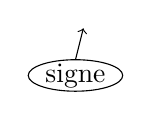
\begin{tikzpicture}\node (s) at (0,0) {\unsure{signe}};\draw (0,0) ellipse (.6 and .2);\draw[->] (0,.2)--(.1,.6);\end{tikzpicture}}}
i.e.
\[
g(x)(y)=-\psi(y)x,
\]
mais c'est aussi OK.

Ceci vu, l'isom. d'ext. $g$ définit
\[
\operatorname{Quad}(E,L^{\otimes2})\simeq\operatorname{Quad}(\mathcal A,\mathcal O)
\]
\[
\deleted{\unsure{\operatorname{Quad}(E)}\otimes L^{\otimes2}\ \unsure{\simeq}\ \unsure{\mathcal A^{\otimes2}}}.
\]
\uline{dès que $\unsure{\varphi}$ est iso}, \uline{$N$} et \uline{$Q$ se \unsure{correspondent|correspondant}}.
\margin{\unsure{lorsque} $E$ provient d'un \unsure{truc du type}, d'où $N$ sur $\mathcal A$, $Q$ sur $E$. \unsure{dans}}
Pour le prouver, \unsure{OS|on} $E$ scindé en
\[
E\simeq L\oplus\underline{\mathcal O}.x_0
\]
d'où
\[
\mathcal A\simeq\underline{\mathcal O}\oplus L^\vee
\qquad\text{i.e. }\mathcal A\otimes L\simeq L\oplus\underbrace{L\otimes L^\vee}_{\underline{\mathcal O}_X}.
\]
\mspage{96}

\scanpage{98}
et l'isom $E\longrightarrow\mathcal A\otimes L$ respecte les décompositions en somme directe
\diagram{\begin{tikzcd}
\underline E={} & \underline L \arrow[d,"-\mathrm{id}_L"'] & \oplus & \underline{\mathcal O}.x_0 \arrow[d,no head,"\mathrm{id}"]\\
\mathcal A\otimes L\simeq{} & \underline L & \oplus & \underline{\mathcal O}.
\end{tikzcd}}
Si donc $Q$ est donné par
\[
Q(\underbrace{u}_{\in\Gamma L}+\lambda x_0)=u^2+\lambda\deleted{\unsure{x}}\langle u,\underbrace{b}_{\in\Gamma L}\rangle+\lambda^2\underbrace{c}_{\in\Gamma L^{\otimes2}},
\]
le signe $-\mathrm{id}_L$ dans les diagrammes précédents implique que l'on aura
\[
N(\underbrace{v}_{\in\Gamma L^\vee}+\lambda1)=\unsure{\lambda^2}\ \deleted{\unsure{+}}\unsure{-}\lambda\langle v,b\rangle+\langle v^2,c\rangle
\]
La formule
\[
\boxed{Q_N(\varphi_N(x))=-N(x)\delta_N}
\]
(\unsure{On donne un sens aux deux symboles pour : l'argument $N$ variable}\ldots) est bien sûr valable dans le contexte général d'un mod. loc. libre $A$ \inserted{de rg $2$} \deleted{et d'} une forme quadratique \deleted{\unsure{inut.}} $N$ dessus, sans autre donnée.
\figure{\begin{tikzpicture}\draw (0,0) .. controls (.12,-.40) and (.20,-.68) .. (.34,-.86);\end{tikzpicture}}
\mspage{97}

\scanpage{99}
Comme $\mathcal A_i\simeq E_i\otimes L_i^\vee$, $\mathcal A\unsure{\otimes|\simeq}E\otimes L^\vee$, on a
\[
E\otimes L^\vee\longleftrightarrow(E_1\otimes L_1^\vee)\otimes(E_2\otimes L_2^\vee)
\]
et comme $L^\vee\simeq L_1^\vee\otimes L_2^\vee$, on en déduit également
\[
E\xrightarrow{i}E_1\otimes E_2
\]
qui est une sorte de transposé de $E_1\otimes E_2\longrightarrow E$.
\margin{$x_1\otimes x_2\mapsto x_1*x_2$;}
\deleted{Pour expliciter $i$, il faut donner les deux composés
$\inserted{\alpha=}i\circ *$, $\inserted{\beta=}i\circ\mathrm{inj}$,
en sorte que $\alpha\circ\mathrm{inc}=2\beta$.}
\deleted{\diagram{\begin{tikzcd}[column sep=large]
E_1\otimes E_2 \arrow[dr,"*"] \arrow[rr,bend left=25,"?"] & & E_1\otimes E_2\\
\begin{array}{c}L_1\otimes E_2\oplus E_1\otimes L_2\\E_1*_0E_2\end{array} \arrow[u,hook,"\mathrm{inc}"] \arrow[drr,no head,"\deleted{\unsure{\mathrm{proj}}}"'] & E \arrow[ur,"i"] & \\
& L_1\otimes L_2 \arrow[u,hook,"\mathrm{inj}"] \arrow[uur,bend right=25,"?\ \text{i.e. can.}"'] &
\end{tikzcd}}}
\deleted{\deleted{Je pense} on voudra $L_1\otimes L_2\longrightarrow E_1\otimes E_2$ inclusion canonique, donc un \unsure{hom}}
\deleted{\diagram{\begin{tikzcd}
E_1\otimes_0 E_2\;\deleted{\unsure{L_2}} \arrow[r,no head] & \unsure{E_1\otimes L_2}\subset E_1\otimes E_2\\
E_1\otimes E_2 \arrow[u,no head,"\unsure{\cap}"] \arrow[ur,dashed,"?"'] &
\end{tikzcd}}}
\deleted{(pour $\boxed{\uuline{\unsure{\chi}=2.}}$),}
\deleted{\deleted{Je pense} Considérons les inv. canoniques $\sigma_1,\sigma_2$ de $E_1$, de $E_2$, d'où $\sigma=\sigma_1\otimes\sigma_2$ de $\unsure{E}$, noté $\xi\mapsto\bar\xi$. Je pense à l'hom
\[
\xi\longmapsto\xi+\bar\xi
\]
donc
\[
\begin{aligned}
x_1\otimes x_2&\longmapsto x_1\otimes x_2+\bar x_1\otimes\bar x_2\\
&=x_1\otimes x_2+(\unsure{\overline T_1|\varpi_1}\inserted{\psi_1(x_1)}-x_1)\otimes(\unsure{\overline T_2|\varpi_2}\inserted{\psi_2(x_2)}-x_2).
\end{aligned}
\]
Si $x_1=u_1\in\Gamma L_1$, alors on trouve $\bar x_1=-u_1$,
\[
u_1\otimes x_2\longmapsto u_1\otimes x_2+(-u_1)(\unsure{\overline T_2|\varpi_2}\psi_2(x_2)-x_2)
\]
}
\mspage{98}

\scanpage{100}
Considérons, d'ailleurs deux torseurs $\unsure{\chi|\gamma}$-trivialisés $\deleted{\unsure{P}}P_1$, $P_2$ sur les mod. \uline{inv.} $L_1,L_2$, l'homomorphisme can
\diagram{\begin{tikzcd}[column sep=large]
E_1\otimes E_2 \arrow[r,no head,"x_1\otimes x_2\mapsto x_1*x_2"] \arrow[d,phantom,"\wr"] & E_1\unsure{*|\wedge}E_2=E \arrow[d,phantom,"\wr"]\\
(\mathcal A_1\otimes L_1)\otimes(\mathcal A_2\otimes L_2) & \mathcal A\otimes L
\end{tikzcd}}
avec $L=L_1\otimes L_2$.
On en déduit
\[
\mathcal A_1\otimes\mathcal A_2\xrightarrow{\tau_A}\mathcal A
\]
qu'on va aussi dénoter
\[
\xi_1\otimes\xi_2\longmapsto\xi_1*\xi_2
\]
et qu'on voudrait étudier. On a d'autre part, dans le cas $\chi=2$ et quand $\unsure{P_1},P_2$ correspondent à des \deleted{$\mathcal A\longrightarrow$} rev. quadratiques $X_1,X_2$ de $X$, alors $E$ à un rev. quad. de \unsure{type}
\[
\mathcal X=X_1\wedge X_2
\]
de $X$, à cause de
\[
X_1\times X_2\longrightarrow\mathcal X
\]
induit par $(*)$, un hom ``transposé''
\[
\mathcal A\xrightarrow{i_A}\mathcal A_1\otimes\mathcal A_2
\]
mais c'est simplement le transposé de
\[
E_1\otimes E_2\xrightarrow[\inserted{x_1\otimes x_2\mapsto x_1*x_2}]{\tau_E}E
\]
qui a \inserted{donc} un sens sans utiliser les structures de rev. i.e. les formes quadratiques $Q_1,Q_2$, ni \unsure{les conditions|la condition} $\chi=2$.
\mspage{99}

\scanpage{101}
Je préfère faire les calculs du côté de $\mathcal A_1,\mathcal A_2$.
On peut expliciter la construction de $\mathcal A$ ainsi
\diagram{\begin{tikzcd}[column sep=large]
0 \arrow[r] & \overbrace{\mathcal A_1\unsure{\oplus|\amalg}_{\underline{\mathcal O}}\mathcal A_2}^{=\mathcal A_1\otimes_0\mathcal A_2} \arrow[r,no head] \arrow[d,"\tau"'] & \mathcal A_1\otimes\mathcal A_2 \arrow[r] \arrow[d,no head,"\unsure{\uparrow|\downarrow}"] & L_1^\vee\otimes L_2^\vee \arrow[r,no head] \arrow[d,equal] & 0\\
0 \arrow[r] & \underline{\mathcal O} \arrow[r] & \mathcal A \arrow[r] & L_1^\vee\otimes L_2^\vee \arrow[r] & 0
\end{tikzcd}}
\inserted{Trace réduite, qui est $\operatorname{Tr}_{A_1}$, $\operatorname{Tr}_{A_2}$ sur les deux composantes.}
$\mathcal A$ \inserted{$=\mathcal A_1*\mathcal A_2$} est l'ext. de $L_1^\vee\otimes L_2^\vee$ par $\underline{\mathcal O}$, déduite de l'extension $\mathcal A_1\otimes\mathcal A_2$ de $L_1^\vee\otimes L_2^\vee$ par $\mathcal A_1\otimes_0\mathcal A_2$, par l'hom $\tau$
\[
\mathcal A_1\amalg_{\underline{\mathcal O}}\mathcal A_2\mathrel{-\!\!-\!\!-}\mathcal O.
\]
Pour donner l'hom
\[
\mathcal A\longrightarrow\mathcal A_1\otimes\mathcal A_2
\]
c'est se donner séparément
\[
\underline{\mathcal O}\mathrel{-\!\!-\!\!-}\mathcal A_1\otimes\mathcal A_2
\]
\margin{(on prendra l'inclusion canonique $\lambda\mapsto\lambda.e_{A_1}\otimes e_{A_2}$}
et
\[
\mathcal A_1\otimes\mathcal A_2\xrightarrow[\inserted{x_1\otimes x_2\mapsto i(x_1*x_2)}]{\unsure{\varphi}}\mathcal A_1\otimes\mathcal A_2
\]
tel que les composés sur
\diagram{\begin{tikzcd}
& \mathcal O\\
\mathcal A_1\otimes_0\mathcal A_2=\mathcal A_1\oplus_{\mathcal O}\mathcal A_2 \arrow[ur] \arrow[dr] &\\
& \mathcal A_1\otimes\mathcal A_2
\end{tikzcd}}
soient égaux. On prendra
\mspage{100}

\scanpage{102}
\[
\xi^{\unsure{\natural|\flat}}=\xi+\bar\xi\deleted{^{\unsure{\natural}}}
\qquad\text{pour }\xi\in\mathcal A_1\otimes\mathcal A_2,
\]
en \unsure{supposant|supprimant} maintenant $\unsure{\chi}=2$ i.e. qu'on a
\[
\begin{aligned}
x_1&\mapsto\bar x_1=\deleted{\unsure{\overline T_1}\psi_1(x_1)}\inserted{\operatorname{Tr}_1(x_1)}-x_1,\\
x_2&\mapsto\bar x_2=\deleted{\unsure{\overline T_2}\psi_2(x_2)}\inserted{\operatorname{Tr}_2(x_2)e_2}-x_2
\end{aligned}
\]
sur $\mathcal A_1,\mathcal A_2$, donc
\[
\xi\mapsto\bar\xi,\quad x_1\otimes x_2\mapsto\overline{x_1\otimes x_2}\overset{\mathrm{def}}=\bar x_1\otimes\bar x_2
\]
sur $\mathcal A_1\otimes\mathcal A_2$. On aura donc, si $\xi\in\mathcal A_1$ i.e. $\xi=x_1\otimes e_2$
\[
\xi^{\unsure{\natural}}=(x_1\otimes1)^{\unsure{\natural}}=(x_1+\bar x_1)\deleted{\unsure{^{\natural}}}\otimes e_2=\operatorname{Tr}_1(x_1)e_1\otimes e_2
\]
c'est OK.

\uline{NB} Si \deleted{\unsure{la structure}} sur $X_0=V(2.1_X)\subset X$ (lieu de car. $2$), en tt pt de $X_0$ l'une des deux structures $E_1,E_2$ est étale, alors $\mathcal A\hookrightarrow\mathcal A_1\otimes\mathcal A_2$ est univ injectif, et a pour image
\[
(\mathcal A_1\otimes\mathcal A_2)^{\unsure{\natural}}=(\mathcal A_1\otimes\mathcal A_2)^{\sigma_1\otimes\sigma_2}.
\]
Ceci posé, on peut \inserted{donc} identifier l'application
\[
(x_1,x_2)\mapsto x_1*x_2:\mathcal A_1\times\mathcal A_2\longrightarrow\mathcal A
\]
ou
\[
x_1\otimes x_2\mapsto x_1*x_2\qquad \mathcal A_1\otimes\mathcal A_2\longrightarrow\mathcal A
\]
à des applications à valeurs dans $(\mathcal A_1\otimes\mathcal A_2)^{\unsure{\natural}}$.
\unsure{En tant que telle} elle est simplement \unsure{définie} comme \uline{l'application trace} pour $\sigma_1\otimes\sigma_2$.

Quand $\mathcal A_1,\mathcal A_2$ sont des alg. de \unsure{rev. quad.|rev. qu. ét.}, il s'agit bien de trace au sens habituel.
Mais cette trace, sans cond. de car. $\ne2$ \unsure{etc.},
\mspage{101}

\scanpage{103}
elle \unsure{vaut} sur $1,U_1,U_2$ par
\[
1\longmapsto2\deleted{\unsure{e}},\qquad U_1\mapsto-b_1,\quad U_2\mapsto-b_2
\]
\unsure{chute} en $\Gamma\underline{\mathcal O}\subset\Gamma\mathcal A$, il reste à trouver l'image de $U_1\otimes U_2$, c'est donc un élément de $\mathcal A$ dont l'image dans $(\mathcal A_1\otimes\mathcal A_2)^{\unsure{\natural}}$ est
\[
U_1\otimes U_2+\underbrace{\bar U_1\otimes\bar U_2}_{(-b_1\unsure{-|+}U_1)\otimes(-b_2-U_2)}=\underbrace{2U_1U_2+b_1U_2+b_2U_1}_{\text{image de }U}+b_1b_2
\]
\deleted{\unsure{donc}} donc il y a lieu de prendre
\[
U_1*U_2=U+b_1b_2
\]
Mais il faut maintenant définir une application
\[
N_{\mathcal A_1\otimes\mathcal A_2/\mathcal A}:\mathcal A_1\otimes\mathcal A_2\unsure{\mathrel{-\!\!-\!\!-}|\longrightarrow}\mathcal A
\]
application quadratique, dont la valeur en $z$ serait, essentiellement, $z\bar z$, mais ``\unsure{remonté|remontée}'' à $\mathcal A$.
L'application bil. associée serait
\[
(u,v)\longmapsto u\bar v+v\bar u=\operatorname{Tr}_N(u\bar v)
\]
déjà connue.

Donc il faut se donner les \unsure{autres} valeurs de $N$, et de $\varphi_N$, sur les éléments de la base $1,U_1,U_2,U_1\otimes U_2$ de $\mathcal A_1\otimes\mathcal A_2$. On devrait avoir
\[
\begin{array}{c}
N_{\mathcal A}(x_1\otimes x_2)=N_1(x_1)N(x_2)\in\Gamma\mathcal O\subset\Gamma\mathcal A\\
\Vert\\
(x_1\otimes x_2)(\bar x_1\otimes\bar x_2)\\
\Vert\\
(x_1\bar x_1)\otimes(x_2\bar x_2)
\end{array}
\]
On \unsure{peut écrire}
\[
N(1)=1,\quad N(U_1)=N_1(U_1)=c_1,\quad N(U_2)=N_2(U_2)=c_2
\]
\[
N(U_1\otimes U_2)=c_1c_2
\]
\mspage{102}

\scanpage{104}
peut se définir comme à \uline{valeurs dans} $\mathcal A$ (et non seulement comme à val. dans $(\mathcal A_1\otimes\mathcal A_2)^{\unsure{\natural}}$, alors qu'on ne sait pas si $\mathcal A\longrightarrow(\mathcal A_1\otimes\mathcal A_2)^{\unsure{\natural}}$ est \inserted{seulement} injectif, ni d'ailleurs surjectif).

On doit pouvoir définir de même une norme, définie universellement par la condition que son image dans $(\mathcal A_1\otimes\mathcal A_2)^{\unsure{\natural}}$ soit $\xi.\bar\xi$.
Choisissons les bases
\[
(1,\unsure{U_1})\text{ de }\mathcal A_1,\qquad (1,U_2)\text{ de }\mathcal A_2
\]
donc
\[
\mathcal A_1=\mathcal O[U_1]/(U_1^2+b_1U_1+c_1),\qquad
\mathcal A_2=\mathcal O[U_2]/(U_2^2+b_2U_2+c_2),
\]
on aura
\[
\left\{\begin{aligned}
\mathcal A_1\otimes\mathcal A_2&=\mathcal O[U_1,U_2]/(U_1^2+b_1U_1+c_1,\ U_2^2+b_2U_2+c_2)\\
\mathcal A&\simeq\mathcal O[U]/(U^2+bU+c)
\end{aligned}\right.
\]
avec
\[
\left\{\begin{aligned}
b&=b_1b_2\\
c&=b_1^2c_2+b_2^2c_1-4c_1c_2
\end{aligned}\right.
\]
et $\mathcal A\longrightarrow\mathcal A_1\otimes\mathcal A_2$ est donné par
\[
U\longmapsto2U_1U_2+b_1U_2+b_2U_1
\]
Explicitons
\[
\mathcal A_1\otimes\mathcal A_2\xrightarrow[\inserted{x_1\otimes x_2\mapsto x_1*x_2}]{\tau}\mathcal A
\]
il suffit de trouver les images de $1,U_1\otimes1,1\otimes U_2,U_1\unsure{\otimes U_2}$.
\margin{c'est donc ce qui \unsure{joue} le \unsure{rôle} d'une \unsure{trace} de $\mathcal A_1\otimes\mathcal A_2$ \unsure{en disposant des}}
On aura bien sûr
\[
\deleted{\unsure{x_1*}}\quad x_1*e_1=\operatorname{Tr}_1(x_1).1_{\mathcal A}
\qquad e_1*x_2=\operatorname{Tr}_2(x_2).1_{\mathcal A}
\]
\margin{Ce qui définit $*$ sur $\mathcal A_1\unsure{\oplus|\amalg}\mathcal A_2\subset\mathcal A_1\otimes\mathcal A_2$.}
\mspage{103}

\scanpage{105}
\uline{Proposition} Soient $A_1,A_2$ des alg. quadratiques sur $O$, et $A=A_1\wedge A_2$. \deleted{On a alors}.

1) \deleted{On a \unsure{alors}} L'hom canonique
\[
 A_1\otimes A_2\xrightarrow{\deleted{\unsure{\tau}}\,\inserted{\operatorname{Tr}_{A_1\otimes A_2/A}}}A
\]
(défini par la construction de $A$ comme ext. de $L_1^\vee\otimes L_2^\vee$ par $\underline O$, déduite de l'extension \inserted{$A_1\otimes A_2$} de $L_1^\vee\otimes L_2^\vee$ par $A_1\unsure{\oplus_{\underline O}|\amalg_{\underline O}}A_2\subset A$, \inserted{$A_1\oplus_{\underline O}A_2$} et de l'hom
\[
 A_1\oplus_{\underline O}A_2\xrightarrow[\substack{\text{donné par}\\ \operatorname{Tr}_{A_1}\text{ et }\operatorname{Tr}_{A_2}\\\text{sur les deux sommants}}]{\operatorname{Tr}}\underline O,
\]
\margin{\uline{NB} On a
$\operatorname{Tr}\,(\sigma_1\otimes\operatorname{id}_{A_2})(\xi)=\deleted{\unsure{\overline{\operatorname{Tr}(\xi)}}}\operatorname{Tr}\,(\operatorname{id}_{A_1}\otimes\sigma_2)(\xi)
=\deleted{\unsure{\sigma_A}}\overline{\operatorname{Tr}\xi}$, d'où
$\operatorname{Tr}(\bar\xi)=\operatorname{Tr}(\xi)$ où $\bar\xi=(\sigma_1\otimes\sigma_2)\unsure{_{A_1\otimes_{\underline O}A_2}}(\xi)$.}
sera considéré comme \unsure{``un hom. trace''|un hom. trace}.
Son composé avec l'hom can.
\[
 A\mathrel{-\!\!-\!\!-}A_1\otimes A_2
\]
(qui a \unsure{tendance} à être univ. injectif, cf. plus haut) \deleted{\unsure{est}} n'est autre que
\[
 \xi\longmapsto\xi+\bar\xi,\qquad\text{i.e.}\quad
 \boxed{i\bigl(\operatorname{Tr}_{A_1\otimes A_2/A}(\xi)\bigr)=\xi+\bar\xi}
\]
\[
 \bar\xi=\sigma_1\otimes\sigma_2(\xi)
\]
\margin{On a aussi $\boxed{\operatorname{Tr}_{A_1\otimes A_2/A}(i(\eta))=2\eta}$ pour $\eta\in\Gamma A$.}
$\sigma_1,\sigma_2$ les involutions canoniques de $A_1,A_2$
\[
 x_1\longmapsto\operatorname{Tr}_{A_1}(x_1)-x_1,\qquad
 x_2\longmapsto\operatorname{Tr}_{A_2}(x_2)-x_2.
\]

2) Il existe sur $A_1\otimes A_2$ une application quadratique unique, à val. dans $A$, notée
\[
 N=N_{A_1\otimes A_2/A},
\]
\mspage{104}

\scanpage{106}
ayant les propriétés suivantes
\[
\text{a)}\quad N(x_1\otimes x_2)=N_{A_1}(x_1)N_{A_2}(x_2)
\qquad\begin{gathered}x_1\in\Gamma A_1\\x_2\in\Gamma A_2\end{gathered}
\]
\[
\text{b)}\quad \varphi_N(\xi,\eta)=\operatorname{Tr}_{A_1\otimes A_2/A}(\xi\bar\eta)
\]
\deleted{On aura de}
i.e.
\[
 \deleted{\unsure{\varphi}}N(\xi+\eta)=N(\xi)+N(\eta)+\operatorname{Tr}(\xi\bar\eta)
\]
On \deleted{aura alors}, pour $\forall\xi\in A_1\otimes A_2$
\[
 \boxed{i(N(\xi))=\xi\bar\xi}
\]
\[
\left\{\boxed{\begin{gathered}
 N(\sigma_1\otimes\operatorname{id}_{A_2}(\xi))=N(\operatorname{id}_{\unsure{A_2|A_1}}\otimes\sigma_2(\xi))=\overline{N(\xi)}\\
 N(\bar\xi)=N(\xi)
\end{gathered}}\right.
\]
\margin{\unsure{Noter} aussi $\boxed{N_{A_1\otimes A_2/A}(i(\eta))=\eta^2}$.}
De plus, on a
\[
 \boxed{N_{A/O}\bigl(N_{A_1\otimes A_2/A}(\xi)\bigr)=N_{A_1\otimes A_2/O}(\xi)}
\]
sans compter la formule plus bénigne
\[
 \boxed{\operatorname{Tr}_{A/O}\bigl(\operatorname{Tr}_{A_1\otimes A_2/A}(\xi)\bigr)=\operatorname{Tr}_{A_1\otimes A_2/O}(\xi)}
\]
Prouvons p.ex. la première des deux dernières. La \deleted{deuxième}
Posons
\[
 \sigma_1=\sigma_{A_1}\otimes\operatorname{id}_{A_2},\qquad
 \sigma_2=\operatorname{id}_{A_1}\otimes\sigma_2,
 \qquad\sigma_3=\sigma_1\sigma_2
\]
\deleted{\unsure{\xi}}\deleted{Soit} $\xi=\xi_0\in A$, \deleted{on doit vérifier}
\inserted{$\xi_i=\sigma_i(\xi)$,}
on \unsure{constate} qu'on \unsure{ait|a}
\figure{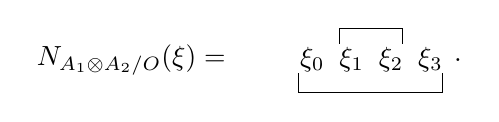
\begin{tikzpicture}
\node at (0,0) {$N_{A_1\otimes A_2/O}(\xi)=$};
\node at (2.3,0) {$\xi_0$};
\node at (2.8,0) {$\xi_1$};
\node at (3.3,0) {$\xi_2$};
\node at (3.8,0) {$\xi_3$};
\node at (4.15,0) {$.$};
\draw (2.12,-.17)--(2.12,-.42)--(3.95,-.42)--(3.95,-.17);
\draw (2.65,.2)--(2.65,.4)--(3.45,.4)--(3.45,.2);
\end{tikzpicture}}
\mspage{105}

\scanpage{107}
Or le deuxième est $\xi_0\underset{\substack{\Vert\\\xi_3}}{\bar\xi_0}\,\xi_1\underset{\substack{\Vert\\\xi_2}}{\bar\xi_1}$, or
\[
 \xi_0\bar\xi_0\overset{\unsure{!}}{=}N_{A_1\otimes A_2/A}(\xi_0)
\]
\[
 \xi_1\bar\xi_1=N_{A_1\otimes A_2/A}\left(\underset{\substack{\Vert\\\sigma_1(\xi_0)}}{\xi_1}\right)
 =\overline{N_{A_1\otimes A_2/A}(\xi_0)}
\]
donc \deleted{\unsure{soit}} $N=N_{A_1\otimes A_2/A}(\xi_0)$, on trouve
\[
 N\bar N=N_{A/O}(N)\qquad\text{OK}.
\]
\figure{\begin{tikzpicture}\draw[->] (0,0)--(1.5,0);\end{tikzpicture}}

On va axiomatiser la situation de \deleted{$\unsure{A_1\ A_1,O}$} $\operatorname{Tr}_{A_1\otimes A_2/A}$ et $N_{A_1\otimes A_2/A}$, \unsure{en oubliant la} situation d'un anneau de base $k$, \inserted{et} d'une ``$k$-algèbre $A$ qui ``se comporte comme si c'était une algèbre quadratique sur $k$'' (i.e. loc. libre de rang $2$). Mais on ne suppose ni que $A$ soit loc. libre \deleted{\unsure{sur}}\inserted{ni même plat} / $k$, ni que
\[
 \alpha:k\longrightarrow A\qquad\lambda\mathrel{-}\lambda.1_A
\]
soit injective. Au lieu de cela, on suppose données deux applications
\[
 \begin{array}{lll}
 t_{A/k}=t:A\mathrel{-\!\!-\!\!-}k&\text{trace relative},\\
 n_{A/k}=n:A\mathrel{-\!\!-\!\!-}k&\text{norme relative},
 \end{array}
\]
satisfaisant les conditions suivantes

\textcircled{a} $t$ est linéaire, $n$ est quadratique et $t$ se déduit de $n$, comme \inserted{$t(x)=\varphi_n(x,1)$} $\varphi_n$ forme bil. ass. à $n$
donc on a
\[
 \deleted{\unsure{c'est}}\boxed{n(x+\lambda 1_A)=n(x)+\lambda^2\underset{\substack{\Vert\\1\ \text{cf. ci-dessous b)}}}{n(1)}+\lambda t(x)}
\]
\mspage{106}

\scanpage{108}
\deleted{D'autre part, la forme} \inserted{\uline{NB} On verra plus bas comment la forme bil. $\varphi_n$} s'explicite \unsure{en termes de $t$ par $\tau$}.

\textcircled{b}
\[
 \boxed{\unsure{N|n}(1)=1,\qquad n(xy)=n(x)n(y)}
\]
i.e. $n$ est un hom de monoïdes unitaires $A^\times\longrightarrow k^\times$
\inserted{D'où via a), pour $x=1$ $\boxed{t(1)=2}$.}
\deleted{\unsure{Posons}}\deleted{\unsure{Posons}}

\textcircled{\unsure{c|b}}
Posons $\tau(f)=\alpha(t(f))$, et considérons l'application
\[
 \sigma:f\longmapsto\bar f=\tau(f)-f
\]
\deleted{\unsure{On veut que cette application soit}}
On a
\[
 \tau(\bar f)=\tau(f)\underbrace{\tau(1)}_{2}-\tau(f)=\tau(f)
\]
d'où
\[
 (\bar f)\bar{\phantom f}=\tau(\bar f)-\bar f=f
\]
i.e. \deleted{\unsure{on a}}
\[
 \sigma^2=\operatorname{id}_A.
\]
\margin{Notons que par définition $\boxed{\tau(f)\overset{\mathrm{def}}{=}\alpha(t(f))=f+\bar f}$ et on a $\bar1=1$.}
Ceci posé, on veut que l'on ait

\uline{$1^\circ$}) $\sigma$ est un autom. d'algèbre, i.e.
\[
 \boxed{\sigma(xy)=\sigma(x)\sigma(y)}\qquad x,y\in A
\]
ce qui s'explicite ainsi
\[
 2xy=\underset{\substack{\Vert\\\varphi_n(x,\bar y)\ \longrightarrow\ \text{voir d) ci-dessous}}}{\tau(xy)}\inserted{-\tau(x)\tau(y)}+x\tau(y)+y\tau(x)
\]
\margin{\unsure{comb. lin.|cond. lin.} (à coeff. dans $k$) de $1,x,y$}
\uline{NB} Au facteur $2$ près (qui n'est gênant que \deleted{\unsure{en car.}} si $2$ n'est pas inv. dans $k$), on voit donc que la structure d'algèbre de $A$ est connue quand on connaît $A$ en tant que $k$-module, avec l'élément $1_A$ (d'où $\alpha:k\mathrel{-}A$ par $\lambda\mapsto\lambda.1_A$) et les appl.
\[
 t:A\longrightarrow k,\qquad n:A\mathrel{-\!\!-\!\!-}k.
\]
\margin{\uline{NB} Quand $\alpha$ est injectif, les formules \unsure{ci-dessous|ci-dessus} $\alpha n(x)=x\bar x$ \unsure{(de $2^\circ$)} impliquent \textcircled{b} \unsure{ci-dessus} $\begin{gathered}n(1)=1\\n(xy)=n(x)n(y)\end{gathered}$ \unsure{qui}.}

$2^\circ$)
\[
 \boxed{\alpha(\unsure{N|n}(x))=x\bar x}
\]
implique
\[
 \alpha(n(x))=\alpha\bigl(\unsure{\overline{n(x)}|n(\bar x)}\bigr),
\]
\figure{\begin{tikzpicture}\draw (0,0) .. controls (0.35,-0.4) and (0.8,-0.3) .. (0.85,0.2) .. controls (1,1) and (2,1.3) .. (2.4,0.95);\end{tikzpicture}}
\unsure{mais en} \deleted{\unsure{voudra que}} fait
\[
 \deleted{\unsure{3^\circ)}}\boxed{n(\bar x)=n(x)}.
\]
Car
\[
 n(\bar x)=n(\deleted{\unsure{t(x)}}\inserted{\lambda}1-x)
 \underset{\text{cf. \textcircled{a}}}{=}
 n(x)+\deleted{\unsure{t(x)^2}}\lambda^2-\lambda t(x)
 \qquad\text{où }\lambda=t(x)
\]
\inserted{avec $\lambda=t(x)$}
donc on a bien $n(\bar x)=n(x)$.
\mspage{107}

\scanpage{109}
La formule ci-dessus pour
\[
 \deleted{\unsure{d'où}}\alpha(n(x))=x\bar x
\]
donne, si on fait $x=y+z$
\[
\begin{aligned}
 \alpha\left(\underbrace{n(y+z)}_{\substack{\Vert\\n(y)+n(z)+\varphi_n(y,z)}}\right)
 &=\deleted{\unsure{\alpha(x\bar x)}}(y+z)\overline{(y+z)}=\\
 &=\underset{\substack{\Vert\\\alpha(n(y))}}{y\bar y}
 +\underset{\alpha(n(z))}{z\bar z}
 +\underbrace{y\bar z+\underbrace{z\bar y}_{=\overline{y\bar z}}}_{\tau(y\bar z)}
\end{aligned}
\]
donc
\[
 \alpha(\varphi_n(y,z))=\deleted{\unsure{\alpha t}}\tau(y\bar z)\qquad\text{i.e.}\quad\alpha(t(y\bar z))
\]
donc si $\alpha$ est injectif, on en déduit
\[
 \boxed{\varphi_n(y,z)=t(y\bar z)}
\]
i.e. la formule d'additivité pour $n$
\[
 \boxed{n(y+z)=n(y)+n(z)+\underset{\substack{\Vert\\t(\bar y z)}}{t(y\bar z)}}
 \qquad\text{car }t(x)=t(\bar x).
\]

Ceci posé, on veut

$3^\circ$) la formule précédente est vraie (sans supposer $\alpha$ injectif\ldots)

$4^\circ$) Une formule facultative, quand $k$ est fini loc. libre de rang \deleted{$\unsure{2}$} $n$ sur un anneau $k_0$, et \deleted{\unsure{alors on supposera}} $A$ loc. libre de rang $2n$ sur $k_0$ (N.B. donc $k_0\mathrel{-\!\!-\!\!-}A$ injectif, mais on ne suppose pas $k\mathrel{-\!\!-\!\!-}A$ injectif).
\[
 \boxed{\left\{\begin{aligned}
 \operatorname{Tr}_{k/k_0}(t(x))&=\operatorname{Tr}_{A/k_0}(x)\\
 N_{k/k_0}(n(x))&=N_{A/k_0}(x)
 \end{aligned}\right.}
\]
\margin{identité entre applic. \uline{linéaires} $A\mathrel{-\!\!-\!\!-}k_0$}
\margin{identité de $(2n)$-formes}
\mspage{108}

\scanpage{110}
Récapitulons le formulaire pour
\diagram{\begin{tikzcd}[column sep=large]
 k\arrow[r,"\deleted{\unsure{\alpha}}\,\alpha"] & A\ (k.\mathrm{alg})\arrow[l,bend left=35,"t"]\arrow[l,bend left=65,"n"]
\end{tikzcd}}
\margin{$\alpha$ hom d'anneaux comm. $\alpha(\lambda)=\lambda.1_A$.
On pose $\tau(x)=\alpha t(x)$, $\unsure{\nu|\gamma}(x)=\alpha n(x)$.}

\textcircled{1} $t$ \unsure{est} $k$-linéaire, $\boxed{t(1_A)=2}$.

\textcircled{2} $x\longmapsto\bar x\overset{\mathrm{def}}{=}\tau(x)-x:A\longrightarrow A$
\margin{(autom. involutif du $k$-\uline{module} $A$, avec $\bar1_A=1_A$)}
est un \uline{automorphisme} d'alg., i.e. on a
\[
 \boxed{\overline{xy}=\bar x\bar y}\qquad\text{i.e.}\quad
 2xy=(\tau(xy)-\tau(x)\tau(y))+\tau(y)x+\tau(x)y
\]

\textcircled{3}
\[
 \boxed{\left\{\begin{aligned}n(\lambda x)&=\lambda^2n(x)\\n(x+y)&=n(x)+n(y)+t(x\bar y)\end{aligned}\right.}
 \qquad\lambda\in k,\ x\in A
\]
i.e. $n$ est quadratique, la forme bil. ass. est \unsure{ici}
\[
 \varphi_n(x,y)=t(x\bar y)
\]

\textcircled{4} $\boxed{n(1)=1}$
\margin{(\uline{NB} compte \deleted{\unsure{dans}} tenu de la formule d'additivité dans $3^\circ$, cela implique $t(1)=2$)}

\textcircled{5} $\boxed{\alpha(n(x))=x\bar x}$\qquad$(x\in A)$
\margin{qui implique $3^\circ,4^\circ$ si $\alpha$ injectif}

\textcircled{6} (\uline{facultatif}), \deleted{\unsure{si}}\inserted{et} (si $k$ loc. libre de rang $n$ sur $k_0$, et $A$ loc. libre de rang $2n$ sur $k_0$)
\[
 \boxed{\begin{aligned}
 \operatorname{Tr}_{k/k_0}(t(x))&=\operatorname{Tr}_{A/k_0}(x)\\
 N_{k/k_0}(n(x))&=N_{A/k_0}(x)
 \end{aligned}}\qquad x\in A
\]
La donnée de \inserted{$A$ sur $k$ avec} $\alpha,t,n$ satisfaisant $1^\circ$ à $5^\circ$ sera appelée algèbre \uline{quasi-quadratique} sur $k$.
On va maintenant \unsure{poursuivre l'étude de la} situation \deleted{\unsure{bi}}\inserted{quasi} \uline{quadratique}
\mspage{109}

\scanpage{111}
Données

a) anneau de base $k$

b) $k$-algèbres $A_1,A_2,A_3,A$

c) Sur chacune des $A_i$, structure quasi-quadratique sur $k$, i.e. on a
\diagram{\begin{tikzcd}A_i\arrow[r,shift left=2,"t_i"]\arrow[r,shift right=2,"n_i"']&k\end{tikzcd}}
\deleted{On pose}
satisfaisant les conditions $1^\circ$ à $5^\circ$ ci-dessus. On \unsure{notera} $a\longrightarrow\bar a$ l'involution canonique de $A_i$,
\[
 \bar a=t_i(a)-a
\]
\deleted{$\unsure{\bar a=\tau_i}$}
(NB on identifie \inserted{par \unsure{abus de} notation} $\lambda\in k$ avec son image dans les $A_i$, sans forcément supposer $k\mathrel{-\!\!-\!\!-}A_i$ injectif\ldots)

d) Des Hom de $k$-algèbres
\diagram{\begin{tikzcd}[column sep=large]
 A_1\arrow[dr,"\alpha_1"']&A_2\arrow[d,"\alpha_2"]&A_3\arrow[dl,"\alpha_3"]\\
 &A&
\end{tikzcd}}
(pas néc. inj.), et des structures d'alg. quasi-quadratiques de $A$ sur les $A_i$
\deleted{\diagram{\begin{tikzcd}[column sep=large]
 &A\arrow[dl,shift right=2,"\unsure{T_1}"']\arrow[dl,shift left=2,"N_1"]\arrow[d,shift right=2,"\unsure{T_2}"']\arrow[d,shift left=2,"N_2"]\\
 A_1&\deleted{A_3}\inserted{\unsure{A_2}}&
\end{tikzcd}}}
\diagram{\begin{tikzcd}[column sep=large]
 &A\arrow[dl,shift right=2,"T_1"']\arrow[dl,shift left=2,"N_1"]\arrow[d,shift right=2,"T_2"']\arrow[d,shift left=2,"N_2"]\arrow[dr,shift right=2,"T_3"']\arrow[dr,shift left=2,"N_3"]&\\
 A_1&A_2&A_3
\end{tikzcd}}
, chacune satisfaisant donc au formulaire ci-dessus de $1^\circ$ à $5^\circ$. De plus, \uline{compatibilités}.
\deleted{
On pose
\[
 \sigma_i(x)=\unsure{T_i|\overline T_i}(x)-x
\]
\margin{$\sigma_i$ est un autom. involutif de $A$}
et on veut que
\[
 \boxed{\sigma_1\sigma_2=\sigma_3,\quad\sigma_2\sigma_3=\sigma_{\unsure{1|3}},\quad\sigma_3\sigma_1=\sigma_2}
\]
i.e. que les $\sigma_i$ sont des involutions qui \uline{commutent} entre elles, et $\boxed{\sigma_1\sigma_2\sigma_3=\operatorname{id}}$
}
\mspage{110}

\scanpage{112}
Considérons un des 6 diagrammes comm.
\diagram{\begin{tikzcd}
A_1 \arrow[r,no head,"\alpha_1"] \arrow[d,no head] & A \arrow[d,no head,"\alpha_2"] \\
k \arrow[r,no head] & A_2
\end{tikzcd}}
on veut que la situation soit, au pt de vue \unsure{raisonnablement bien}, comme si $A_1$ était quadratique sur $k$, et que $A$ en \unsure{soit déduit} par le changement de base $k\mathbin{-}A_2$.
\margin{Mais \unsure{on ne suppose ni les $A_i$ ni $A/A_i$} quadratiques, ni que $A_1,A_2$ \unsure{engendrent $A$}.}
\textcircled{1°}
\[
\boxed{T_2\bigl(\alpha_1(x_1)\deleted{\alpha_2(x_2)}\bigr)=t_1(x_1)\deleted{\alpha_2(x_2)}}
\]
\margin{Ce qui détermine $T_2$ sur $k[A_1,A_2]\subset A$ en termes de $t_1$.}
i.e. on \unsure{exige} un diagramme comm.
\diagram{\begin{tikzcd}
A_1\otimes_k A_2 \arrow[r,no head] \arrow[d,"t_1\otimes\mathrm{id}_{A_2}"'] & A \arrow[d,"\unsure{T_1|T_2}"] \\
A_2 \arrow[r,equal] & A_2
\end{tikzcd}}
\margin{NB. $A_1\otimes A_2\mathbin{-}A$ n'est pas supposé injectif, mais que $t_1\otimes\mathrm{id}_{A_2}$ s'annule au moins sur le noyau.}
Ceci implique que
\[
\boxed{\sigma_2\bigl(\unsure{\alpha_1(x)}\bigr)=\alpha_1(\bar x)}
\]
i.e. $\sigma_2$ (et aussi $\sigma_3$) ``induit'' sur $A_1$ l'involution donnée $x_1\mathbin{-}\bar x_1$ de $A_1$

On veut une condition similaire pour les normes
\textcircled{2°}
\[
\boxed{\boxed{N_2\bigl(\alpha_1(a_1)\deleted{\unsure{\alpha_2(a_2)}}\bigr)=n_1(a_1)\deleted{\unsure{\alpha_2(a_2)^2}}}}
\]
\mspage{111}

\scanpage{113}
Je dis que cette formule implique que le diagramme similaire au précédent
\diagram{\begin{tikzcd}[column sep=large,row sep=large]
A_1\otimes_k A_2 \arrow[r] \arrow[d,"{\deleted{\unsure{N}}n_1\otimes_k\mathrm{id}_{A_2}}"',"=N_{12}"] & A \arrow[d,no head,"N_2"] \\
A_2 \arrow[r,Rightarrow] & A_2
\end{tikzcd}}
\margin{\figure{\begin{tikzpicture}\draw[->] (.6,.6)--(0,0);\end{tikzpicture}}déduite de la forme $n_1$ par chgt de base $k\mathbin{-}A_2$}
C'est en tous cas vrai pour les éléments de \deleted{la forme} $A_1\otimes_k A_2$ de la forme $x_1\otimes x_2$, car les deux mbs sont alors
\[
 t_1(x_1)\cdot\deleted{\unsure{\alpha_2}}(\unsure{x_2})^{\unsure{2}}
\]
par quadraticité de $N_{1,2},N_2$. Il reste à vérifier qu'on a commutativité pour les \deleted{formes} bil. associées, or pour $N_{12}$ c'est la forme déduite de
\[
 \deleted{(x,y)\longrightarrow}\quad\varphi_{n_1}(x,y)=t_1(x\bar y)\qquad\text{sur }A_1\times A_1,
\]
par chgt. de base $k\longrightarrow A_1$, or on a
\margin{si $x'=\alpha_1(x),\ y'=\alpha_1(y)$}
\[
 \left\{\begin{aligned}
 \deleted{\unsure{x\bar y}}\alpha_1(\bar y)&=\sigma_2(\alpha_1(y))\\
 \underset{\text{dans }A_2}{t_1(x\bar y)}&=T_2(\unsure{\alpha_1}(x\bar y))
 \end{aligned}\right.
\]
donc
\[
 \begin{aligned}
 \varphi_{\unsure{n|n_1}}(x,y)&=T_2(x'\sigma_2(y'))\\
 &\mathrel{\text{''}}\varphi_{N_2}(x',y')
 \end{aligned}\qquad\text{O.K.}
\]
\mspage{112}

\scanpage{114}
\uline{NB} La condition sur $N_2$ implique celle sur $T_2$, en passant aux formes bil. ass., i.e. en l'appliquant pour $a$ \uline{et} pour $1+a$ $(a\in A_1)$.

\textcircled{3°} On veut la condition
\[
 \boxed{\sigma_1\sigma_2\sigma_3=1}
\]
\margin{Cette condition est automatiquement vérifiée sur \unsure{la sous-algèbre} de $A$ engendrée par les $A_i$, car elle est vraie sur chaque $A_i$ (lequel est stable par les $\sigma_i$).}
qui implique que les involutions $\sigma_i$ commutent entre elles (car le produit de 2 d'entre elles est une involution
\[
 \boxed{\begin{aligned}
 \sigma_1\sigma_2&=\sigma_3\\
 \sigma_2\sigma_3&=\sigma_1\\
 \sigma_3\sigma_1&=\sigma_2
 \end{aligned}}
\]
(car pour deux invo. $\sigma$ et $\tau$,
\[
 \sigma\tau=\tau\sigma\quad\Longleftrightarrow\quad(\sigma\tau)^2=\unsure{1}\quad\text{i.e.}\quad\sigma\tau\sigma\tau=1
\]
)

En utilisant $1^\circ)$, \deleted{ceci} \inserted{la condition $\sigma_1\sigma_2\sigma_3=1$} s'explicite par la formule
\[
 2x=T_1(x)+T_2(x)+T_3(x)-\uline{t_2T_2(x)},
\]
non \unsure{apparemment} symétrique, \unsure{mais} elle est équivalente à
\[
 \sigma_2\sigma_3\sigma_1=1,\quad\text{ou}\quad\sigma_3\sigma_1\sigma_2=1,
\]
donc
\[
 \begin{aligned}
 2x&=T_1(x)+T_2(x)+T_3(x)-t_3T_3(x)\\
 2x&=\mathbin{-}\ \mathbin{-}\ \mathbin{-}\ \mathbin{\text{---}}-t_1T_1(x),
 \end{aligned}
\]
donc elles impliquent\unsure{*} la condition
\[
 \boxed{t_1\operatorname{Tr}_1(x)=t_2\operatorname{Tr}_2(x)=t_3\operatorname{Tr}_3(x)}
\]
\margin{du moins si $k\mathbin{-}A$ injectif --- mais on la suppose \unsure{vérifiée} en tous cas.}
(qui ressemble à $6^\circ$ ci-dessus). Si on désigne par $T_{A/k}(x)$ la valeur commune aux trois mbs, on trouve donc la condition
\[
 \boxed{2x=T_1(x)+T_2(x)+T_3(x)-T_{A/k}(x).}
\]
\mspage{113}

\scanpage{115}
\deleted{
\unsure{Sous réserve} que les $\alpha_i:A_i\mathbin{-}A$ soient bien injectifs, elle montre que chacun des $T_i$ est déterminé par les deux autres, via
\[
 \alpha_1T_1(x)=2x+\deleted{\unsure{\alpha_2T_2(x)\alpha_3T_3(x)}}\inserted{T_{A/k}(x)-\alpha_2T_2(x)-\alpha_3T_3(x)}
\]
On s'attend à trouver \deleted{des} formules similaires, multiplicatives
\[
 \boxed{N_{A/k}(x)x^2=N_1(x)N_2(x)N_3(x)}
\]
et
\[
 \deleted{\unsure{N}}\boxed{n_1(N_1(x))=n_2(N_2(x))=n_3(N_3(x))}
\]
}
Mais \deleted{toutes} les \deleted{conditions}\inserted{relations sur les normes} \unsure{se prouvent} aisément, comme \uline{conséquences} de celles sur les traces, i.e. la condition $\sigma_1\sigma_2\sigma_3=1$ sur les $\sigma_i$.

En effet, posons
\[
 x_0=x,\quad x_1=\unsure{T_1|\sigma_1}(x),\quad x_2=\unsure{T_2|\sigma_2}(x),\quad x_3=\unsure{T_3|\sigma_3}(x)
\]
On a alors
\diagram{\[
 \begin{array}{c@{\ :\ }ll}
 \sigma_1&x_0\longleftrightarrow x_1&x_2\longleftrightarrow x_3\\
 \sigma_2&x_0\longleftrightarrow x_2&x_1\unsure{\longrightarrow|\longleftrightarrow}x_3\\
 \sigma_3&x_0\longleftrightarrow x_3,&x_1\longleftarrow x_2
 \end{array}
\]}
d'où
\deleted{\[
 \unsure{n_1|N_1}(N_1(x))=N_1(x)\overline{N_1(x)}=\unsure{x\sigma_2(x\sigma_1(x))}
\]}
\deleted{\[
 N_1(x_1)=\unsure{x_1^2n_1}
\]}
\[
 n_1(N_1(x))\overset{!}{=}\underset{\substack{\text{''}\\x\deleted{\unsure{T}}\sigma_1(x)}}{\underbrace{N_1(x)}}\,\overline{N_1(x)}
 =(x_0x_1)\underbrace{\sigma_2(x_0x_1)}_{x_2x_3}=x_0x_1x_2x_3
\]
et de même pour $n_2(N_2(x)),\ n_3(N_3(x))$. Donc on a l'égalité des $n_i(N_i(x))$ si $k\mathbin{-}A$ est \uline{injectif}. Et on a
\[
 \begin{aligned}
 N_1(x)N_2(x)N_3(x)&=(x_0x_1)(x_0x_2)(x_0x_3)\\
 &=x_0^2\underbrace{(x_0x_1x_2x_3)}_{N_{A/k}(x_0)}=x^2N_{A/k}(x),
 \end{aligned}
\]
O.K.
\mspage{114}

\scanpage{116}
Considérons l'algèbre produit tensoriel
\[
 A_1\otimes A_2\otimes A_3;
\]
\unsure{Via} les $\sigma_{A_i}$, le groupe $\mathbb F_2^3$ opère dessus. Il n'y a pas en général d'opération de ce groupe sur $A$, compatible avec
\[
 \bigotimes A_i\mathbin{-}A,
\]
\deleted{car} il faudrait qu'il y ait p.ex. un autom. $\tau_1$ de $A$ qui induise l'identité sur $A_2,A_3$, et $\sigma_{A_1}$ sur $A_1$; Mais dans les cas les plus simples, $A$ est engendré par $A_2,A_3$, donc $\tau_1$ devrait être l'identité, alors qu'il induit $\sigma_{A_1}$ sur $A_1$, qui ne l'est pas.

Par contre, \deleted{soit}
\[
 \begin{aligned}
 \unsure{\gamma|\Gamma}\deleted{\unsure{=}}&\subset\mathbb F_2^3\\
 &\mathrel{\text{''}}\operatorname{Ker}(\mathbb F_2^3\mathrel{-\!\!-\!\!-}\mathbb F_2)\\
 &(\xi_i)\mathbin{-}\textstyle\sum\xi_i
 \end{aligned}
\]
formé des éléments $(\xi_1,\xi_2,\xi_3)$ tels que le nb des composantes $\ne0$ (i.e. $=1$) soit $0$ ou $2$ i.e. soit pair. \deleted{\unsure{Donc}} il y \deleted{\unsure{en}} a trois éléments non nuls de ce groupe, savoir
\[
 \deleted{(0,0,1)},\qquad\begin{gathered}(0,1,1)\\(1,0,1)\\(1,1,0)\end{gathered}
\]
qui correspondent aux autom
\[
 \begin{aligned}
 \mathrm{id}_{A_1}\otimes\sigma_{A_2}\otimes\sigma_{A_3}&\overset{\mathrm{déf}}{=}\tau_1\\
 \sigma_{A_1}\otimes\mathrm{id}_{A_2}\otimes\sigma_{A_3}&\overset{\mathrm{déf}}{=}\tau_2\\
 \sigma_{A_1}\otimes\sigma_{A_2}\otimes\mathrm{id}_{A_3}&\overset{\mathrm{déf}}{=}\tau_3
 \end{aligned}
\]
\mspage{115}

\scanpage{117}
et \deleted{\unsure{là}} on a une \deleted{bonne} op. de $\unsure{\gamma|\Gamma}$ sur $A$, telle que
\[
 \bigotimes A_i\mathbin{-}A
\]
soit compatible aux deux opérations de $\unsure{\gamma|\Gamma}$, savoir celle qui fait opérer
\[
 \tau_i\quad\text{par}\quad\sigma_{A/A_i}.
\]
\figure{\begin{tikzpicture}\draw[->] (0,.1)--(.12,0)--(.35,.04);\end{tikzpicture}}
\deleted{Considér}
Supposons maintenant que les $A_i$ correspondent \deleted{\unsure{à}} des rev. quadratiques $X_i$ de $X$, donc on a un rev. quadratique
\[
 X_1\wedge X_2\wedge X_3,\qquad\text{d'algèbre }B=A_1\unsure{\wedge|*}A_2\wedge A_3,
\]
et on a
\diagram{\begin{tikzcd}[column sep=large]
X_1\times X_2\times X_3\arrow[r]&X_1\wedge X_2\wedge X_3\\
(x_1,x_2,x_3)\arrow[r,no head]&x_1*x_2*x_3
\end{tikzcd}}
i.e.
\diagram{\begin{tikzcd}B\arrow[r]&A_1\otimes A_2\otimes A_3\end{tikzcd}},
et de façon plus précise, on a
\diagram{\begin{tikzcd}B\arrow[r,no head]&(A_1\otimes A_2\otimes A_3)^{\unsure{\gamma|\Gamma}}\end{tikzcd}}
\margin{invariants sous $\unsure{\gamma|\Gamma}$}
Et même, si on exclut les $x\in X=\operatorname{Spec}(k)$ de \uline{car. 2} tels que deux au moins des $A_i$ soient non étales en ce point, alors l'hom précédent est un \uline{iso}.

On va regarder le composé
\diagram{\begin{tikzcd}B\arrow[r,no head]&A_1\otimes A_{\unsure{2|3}}\otimes A_3\arrow[r,no head]&A\end{tikzcd}}, \deleted{\unsure{i.e.}}
\mspage{116}

\scanpage{118}
i.e., en termes de $\mathcal X=\operatorname{Spec}A$, le composé
\diagram{\begin{tikzcd}[column sep=large]
\mathcal X\arrow[r,no head]&X_1\times_X X_2\times_X X_3\arrow[r]&X_1\wedge X_2\wedge X_3
\end{tikzcd}},
j'ai envie de \unsure{prouver} que \unsure{l'on a un hom|c'est un hom} \uline{constant} i.e. qu'il se factorise par une \uline{section} de $X_1\wedge X_2\wedge X_3$, ce qui signifie aussi que l'hom composé précédent
\diagram{\begin{tikzcd}
B\arrow[rr,"f"]\arrow[dr]&&A\\
&(\bigotimes A_i)^{\unsure{\gamma|\Gamma}}\arrow[ur]&
\end{tikzcd}}
est à valeurs dans $k.1_A$. (Du moins, il y a équivalence quand on suppose $k\mathbin{-}A$ injectif --- c'est ce qu'on va supposer maintenant, pour simplifier.)

Mais on a évidemment
\[
 f(B)\subset A^{\unsure{\gamma|\Gamma}},
\]
et la condition \uline{est vérifiée} si on suppose
\[
 \boxed{A^{\unsure{\gamma|\Gamma}}=k.1_A}.
\]
(C'est là une condition pas tjrs vérifiée, même dans des cas intéressants, à cause de la car. 2. Mais si $2$ est inversible dans $k$, c'est tjrs vrai compte tenu des conditions précédentes).
\mspage{117}

\scanpage{119}
En effet, si $a\in A$, $\sigma_i(a)=a$ signifie
\[
 \deleted{\unsure{T_2}}T_i(a)-\unsure{x|a}=a\qquad\text{i.e.}\qquad2\unsure{x|a}=T_i(\unsure{x|a}),
\]
et si c'est vrai pour $i=1,2,3$ on trouve
\[
 6a=\underbrace{T_1(a)+T_2(a)+T_3(a)}_{\substack{\text{'' cf plus haut}\\2x+T_{A/k}\unsure{x}}}
\]
d'où
\[
 \boxed{4\unsure{x|a}=\deleted{\unsure{a}}T_{A/k}(x)}
\]
ce qui implique, si $2$ inv
\[
 a=\frac14T_{A/k}(a)\in k\qquad\text{O.K.}
\]
\deleted{Dans le cas général on va supposer cette condition $A^{\unsure{\gamma|\Gamma}}=k.1_A$.}

\uline{Proposition} Supposons les $A_i$ des alg. quadratiques \uline{étales}, que $k\longrightarrow A$ soit injectif, que les $\alpha_i(A_i)\subset A$ engendrent l'algèbre $A$ i.e. $\bigotimes A_i\mathbin{-}A$ épi,
(donc $\mathcal X=\operatorname{Spec}A\mathbin{-}X_1\times_k X_2\times_k X_3$ est une immersion fermée) \inserted{enfin $A^{\unsure{\gamma|\Gamma}}=k.1_A$.}
Alors \deleted{la situation}\inserted{les hom}
\deleted{se déduit de la situation \unsure{standart|standard}}
\diagram{\begin{tikzcd}\mathcal X\arrow[r]&X_1\times X_2\end{tikzcd}},
\diagram{\begin{tikzcd}\mathcal X\arrow[r]&X_2\times X_3\end{tikzcd}},
\diagram{\begin{tikzcd}\mathcal X\arrow[r]&X_3\times X_1\end{tikzcd}}
sont des iso. (\unsure{donc} $\mathcal X$ est \unsure{fini} \uline{étale} sur $X=\operatorname{Spec}k$)
Et la situation se déduit \uline{par twist} de celle des 3 ens. à deux élts \deleted{\unsure{I}} $I_1,I_2,I_3$, munis d'une trivialisation $\varepsilon$ de $I_1\wedge I_2\wedge I_3$, et de
\[
 J\subset I_1\times I_2\times I_3,\qquad J=\{(\alpha_1,\alpha_2,\alpha_3)\in I_1\times I_2\times I_3\mid\alpha_1\wedge\alpha_2\wedge\alpha_3=\varepsilon\}.
\]
\mspage{118}

\scanpage{120}
Inversement, \inserted{dans} une telle situation \unsure{twistée} $A$ est une algèbre étale quadratique sur chacun des $A_i$, donc on a une situation biquadratique\inserted{étale}, et de plus les hypothèses du début (en particulier $A^{\unsure{\gamma|\Gamma}}=k.1_A$) sont satisfaites.

\deleted{Il faut} Seule la première partie, directe, demande un peu de soin. \unsure{OPS} $X_1,X_2,X_3$ rev. triviaux, $I_{1X},I_{2X},I_{3X}$, et \deleted{la section}\inserted{la section construite plus haut de $X_1\wedge X_2\wedge X_3=(I_1\wedge I_2\wedge I_3)_X$} \unsure{constante|constants}. \deleted{on} On aura alors
\[
 \mathcal X\subset J_X
\]
et tout résulte du lemme suivant

\uline{Lemme} Soit $\unsure{\gamma|\Gamma}$ un groupe, opérant de façon transitive sur un ens. $J$, et considérons un sous-schéma $\mathcal X$ de $X_J$ \inserted{(où $X=\operatorname{Spec}k$)} qui soit tel que

a) $\mathcal X$ est stable sous $\unsure{\gamma|\Gamma}$, et

b) le composé $k\longrightarrow\Gamma(\unsure{X_J},\mathcal O_{\unsure{X_J}})$ $(\simeq k^J)$ est injectif.

Alors $\mathcal X=X_J$, donc $\mathcal X$ est étale sur $X$ (et fini étale si $J$ est fini)

En effet, soit $j_0\in J$, considérons la composante $X_0$ de $X_J$, $X_{\unsure{j|j_0}}\xrightarrow{\sim}X$, et $\mathcal X_{\unsure{j|j_0}}=X\cap\mathcal X$, il correspond à un sous-schéma fermé de $X$ donc à un idéal $\unsure{\mathfrak a}$ de $k$. À cause de l'\unsure{inv.|action} de
\mspage{119}

\scanpage{121}
$\mathcal X$ sous $\unsure{\gamma|\Gamma}$, et de la transitivité de $\unsure{\gamma|\Gamma}$ sur $J$, on voit que cet idéal $\unsure{\mathfrak a}_j$ ne dépend pas de $j$. D'autre part, l'intersection des $\unsure{\mathfrak a}_j$ est évidemment le noyau de
\[
 \deleted{\unsure{k}}k\longrightarrow\Gamma(\unsure{X_J},\mathcal O_{\unsure{X_J}})\simeq k^J.
\]
Comme celui-ci est nul, on a $\unsure{\mathfrak a}_j=0$ \unsure{pour|puis} $\mathcal X_j=X_j$ donc $\mathcal X=X_J$ O.K.
\figure{\begin{tikzpicture}\draw (0,.15) .. controls (.05,.03) and (.25,0) .. (.3,-.1);\end{tikzpicture}}

Ce résultat vaut sans restriction de caractéristique, mais il concerne la situation doublement étale, \uline{trop} restrictive. J'ai envie de vérifier que dès qu'on a trois rev. quadratiques $X_1,X_2,X_3$ de $X$, et une section $\varepsilon$ de $X_1\wedge X_2\wedge X_3$, sans condition étale, on en déduit sur
\[
 \unsure{X|\mathcal X}=\pi^{-1}(\varepsilon)
\]
\margin{\diagram{\begin{tikzcd}[column sep=large]
\unsure{\subset}X_1\times_X X_2\times_X X_3\arrow[r,"\pi"]&X_1\wedge X_2\wedge X_3
\end{tikzcd}}}
une structure biquadratique \unsure{p.r.} aux $\unsure{X_i}$. Ceci doit généraliser la structure biquadratique can. sur un $X_1\times X_2$, par les applications
\diagram{\begin{tikzcd}[column sep=large]
&X_1\\
X_1\times X_2\arrow[ur]\arrow[r,no head]\arrow[dr]&X_2\\
&X_3=X_1\wedge X_2
\end{tikzcd}},
comme on va le voir \unsure{de fait|de suite}.
\mspage{120}

\scanpage{122}
On va regarder, pour $X_1,X_2,X_3$ fixés, la situation universelle, où la base \inserted{(nouvelle)} sera
\[
 \mathcal X_0=X_1\wedge X_2\wedge X_3,
\]
\deleted{\unsure{où}} muni de \unsure{revêts}
\[
 X_{1\mathcal X_0},\quad X_{2\mathcal X_0},\quad X_{3\mathcal X_0}
\]
\margin{$(X_{i\mathcal X_0}=X_i\times_X\mathcal X_0)$}
et où $\mathcal X$ est $X_1\times X_2\times X_3$, avec
\diagram{\begin{tikzcd}[column sep=large,row sep=large]
&X_{1\mathcal X_0}\arrow[dr]&\\
X_1\times X_2\times X_3\arrow[ur,no head,"(\operatorname{pr}_1,\wedge)"]\arrow[r,no head,"(\operatorname{pr}_2,\wedge)"]\arrow[dr,"(\operatorname{pr}_3,\wedge)"']&X_{2\mathcal X_0}\arrow[r]&\mathcal X_0=\\
&X_{3\mathcal X_0}\arrow[ur]&
\end{tikzcd}}
où \deleted{$\unsure{\pi}$}
\diagram{\begin{tikzcd}[column sep=large]
X_1\times X_2\times X_3\arrow[r,no head]&\mathcal X_0=X_1\wedge X_2\wedge X_3
\end{tikzcd}}
est le morphisme
\[
 \unsure{\alpha_1,\alpha_2,\alpha_3|x_1,x_2,x_3}\longmapsto\unsure{\alpha_1\wedge\alpha_2\wedge\alpha_3|x_1\wedge x_2\wedge x_3}.
\]
\unsure{Une|La} difficulté, c'est que ce morphisme n'est pas même fini loc. libre, ni même plat (mais il est bien surjectif).
\diagram{\begin{tikzcd}[column sep=huge,row sep=large]
B=A_1\otimes_{\mathcal O}A_2\otimes_{\mathcal O}A_3\arrow[r,bend left=65,"\operatorname{Tr}_1"]\arrow[r,bend left=40,"N_1\unsure{?}"]\arrow[r,shift left=1.4ex,"\deleted{\unsure{\operatorname{Tr}_1,N_1}}"]\arrow[r,leftrightarrow,shift right=1.4ex,"2(!)"']&A_1\otimes_{\mathcal O}B_0=B_1\\
B_0\arrow[u,"4(!)","{\text{(\unsure{pas univ. inj.})}}"']\arrow[ur,"2"]&\\
\mathcal O\arrow[u,"2"]\arrow[uu,bend left=40,no head,"8"]&
\end{tikzcd}}
\margin{$B_0=A_1\unsure{\wedge|*}A_2\unsure{\wedge|*}A_3$}
$\operatorname{Tr}_1$ doit être $B_0$-linéaire, $N_1$ $B_0$-quadratique\ldots
\mspage{121}

\scanpage{124}
\diagram{\begin{tikzcd}[column sep=large,row sep=large]
0\arrow[r]&L\arrow[r]\arrow[d,"\alpha"']&E\arrow[r,no head]\arrow[l,bend right=45,"\pi"']\arrow[d,no head,"\beta"]&M\arrow[r,no head]\arrow[l,bend right=45,"\unsure{\varpi|\overline\omega}"']\arrow[d,no head,"\gamma"]&0\\
0\arrow[r,no head]&L'\arrow[r,no head]&E'\arrow[r,no head]\arrow[l,bend left=45,"\pi'"]&M'\arrow[r,no head]\arrow[l,bend left=45,"\unsure{\varpi'|\overline\omega'}"]&0
\end{tikzcd}}
\[
 \alpha\pi(x)\unsure{\equiv|=}\pi'\beta(x)\quad\overset{?}{\Longleftrightarrow}\quad\beta\varpi(y)=\varpi'\gamma(y)\quad ?
\]
\[
 \underbrace{\unsure{\beta|\alpha}\pi(x)\unsure{\equiv|=}\pi'\beta(x)}_{\beta(\unsure{\operatorname{id}}-\varpi)=(\unsure{\operatorname{id}}-\varpi')\beta}
 \quad\Longleftrightarrow\quad\beta\varpi(x)\unsure{\equiv|=}
\]
\[
 \deleted{-\beta\varpi=\unsure{-\varpi'}\beta}
\]
\diagram{\begin{tikzcd}[column sep=large,row sep=large]
E_1\arrow[d]&E_2\arrow[d,no head]&\Rightarrow&E_1\wedge E_2\arrow[r]&E'_{\unsure{1}}\\
E'_1&E'_2&&&
\end{tikzcd}}
\diagram{\begin{tikzcd}[column sep=large,row sep=large]
&E_1\otimes E_2\arrow[r]&E'_1\otimes\unsure{E'_2}\arrow[dr,"\unsure{*}"]&\\
{E_1\otimes L_2,\ L_1\otimes E_2}\arrow[ur]\arrow[dr]&&&\unsure{E'_1}\wedge E'_2\\
&L_1\otimes L_2\arrow[r,no head]&L'_1\otimes L'_2\arrow[ur,"\text{inj. can.}"']&
\end{tikzcd}}
\diagram{\begin{tikzcd}[column sep=large,row sep=huge]
\unsure{x_1|u_1}\otimes u_2\arrow[r,mapsto]\arrow[dr,bend right=40]&\beta_1(x_1)\otimes\alpha_2(u_2)\arrow[r,no head]&\begin{gathered}\beta_1(x_1)*\unsure{\varphi'_2(u_2)}\\=\unsure{\pi'_1\beta_1(x_1)\otimes\alpha'_2(\alpha_2(u_2))}\end{gathered}\\
&\pi_1(x_1)\otimes u_2\arrow[r]&\underbrace{\alpha_1\pi_1(x_1)}_{\pi_1\beta_1(x_1)}\otimes\alpha_2(\unsure{x_1|u_2})
\end{tikzcd}}
\[
 E_1\wedge
\]
\mspage{123}

\scanpage{125}
\mspage{465}
Il me semble que notre époque se caractérise comme celle d'une \unsure{exacerbatic|exacerbation}
à outrance de cette dégradation \unsure{culturelte|culturelle}. Parmi les derniers actes de cette
histoire, il y a ceux, intimement solidaires, de la ``course à l'espace'' entre \unsure{le|les}
deux superpuissances antagonistes (imbues de valeurs essentiellement identiques)
et de la course aux armements (nucléaires notamment). Comme acte ultime et \unsure{dénou|dénoue-}\newline
ment probable de cette évolution forcenée dans les surenchères d'un certain type
de ``force'' ou de ``pouvoir'', on peut prévoir dès à présent quelque holocauste nu-\newline
cléaire (ou autre, il y a l'embarras du choix\ldots) à l'échelle planétaire. Il \unsure{aur|aura}
peut-être ce mérite de résoudre tous les problèmes d'un seul coup et une fois \unsure{po|pour}
toutes\ldots

Mon propos ici n'est pas pourtant de brosser un alléchant tableau de ``fin
du monde'' (on ne m'a pas attendu pour cela), et encore moins de partir en guerre
contre le ``muscle'', ou contre ``le cerveau'' (alias l'``esprit''). Je sais bien que
même mes ``tripes'' n'auraient rien à y gagner! Je tiens à mes muscles et à mon
cerveau, qui me sont bien utiles on s'en doute, comme je tiens aussi à mes ``tri-\newline
pes'', qui ne le sont pas moins. Plutôt, il me semble utile de dire ici en \unsure{quelqu|quelques}
mots (si faire se peut) comment s'est joué dans ma propre personne ce conflit \unsure{pr|pro-}\newline
fond, véhiculé par la culture environnante, entre ces deux types de valeurs. En
termes plus terre à terre, il s'agit aussi de l'historique de mes attitudes
(d'acceptation voire d'exaltation, ou de rejet) de deux\quad a s p e c t s\quad ou
f a c e s\quad également réels et tangibles de ma personne, inséparables et complé-\newline
mentaires par nature, et nullement antagonistes par eux-mêmes. Je pourrais les
appeler\quad ``l' h o m m e''\quad et\quad ``l a\quad f e m m e''\quad en moi, ou aussi (pour
prendre des appellations moins ``chargées'', et qui pour cela offrent moins de ris-\newline
que d'induire en erreur), le ``y a n g''\quad et le\quad ``y i n''.

Il semblerait que chez la plupart des personnes, les ``jeux sont faits'' dès
la petite enfance, où se mettent en place les mécanismes essentiels qui, pendant
la vie entière, vont dominer en silence, avec une efficacité d'automate parfaite-\newline
ment au point, attitudes et comportements. Au coeur de ces mécanismes sont ceux
d'affirmation ou de rejet de tels et tels traits en nous, ou de telles pulsions
profondes, à ``signature'' soit yang soit yin, ou de tels et tels ``paquets'' de
traits et de pulsions à signature donnée, voire même du paquet ``yang'' ou du pa-\newline
quet ``yin'' tout entier. Ce sont ces mécanismes qui, dans une très large mesure,
déterminent tous les autres mécanismes de choix (affirmation ou rejet) \unsure{structuran|structurant}
notre ``moi''.
\mspage{124}

\scanpage{126}
\diagram{\begin{tikzcd}[column sep=large,row sep=large]
\mathcal E_{(p_1,q_1),(p_2,q_2)}=(M_1\otimes M_2)\oplus(L_1\otimes L_2)\arrow[rr,no head,"T_U"]\arrow[dd,Rightarrow,"T_{-\gamma b}"']&&\mathcal E_{(p'_1,q'_1),(p'_2,q'_2)}\arrow[dd,no head,"T_{-\gamma b'}"]\\
&\text{\figure{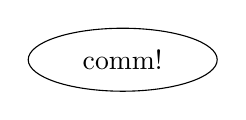
\begin{tikzpicture}\draw (0,0) ellipse (1.2 and .4);\node at (0,0) {comm!};\end{tikzpicture}}}&\\
\mathcal E\arrow[rr,"T_{-U}"']&&\mathcal E
\end{tikzcd}}
\[
 b'=b\deleted{\unsure{i}}\unsure{+|-}\chi U
\]
\[
 U-\gamma b'=U-\gamma b\unsure{-|+}\gamma\chi U=-U-\gamma b
\]
car
\figure{\begin{tikzpicture}\draw (0,.5) .. controls (0,.2) and (-.4,.1) .. (-.4,-.2);\end{tikzpicture}}

d'où un iso d'ext. $\chi$-\unsure{scindées}
\[
 E_1\vee E_2\simeq E_1\wedge E_2
\]
\[
 E'_1\vee E'_2\simeq E'_1\wedge E'_2
\]
\unsure{Je dis qu'il est fonctoriel pour les} \uuline{iso}) : c'est clair par construction.
Mais il y a aussi une notion d'\uuline{hom} d'ext. $\chi$-\unsure{scindées}. Ça marche aussi
\diagram{\begin{tikzcd}[column sep=small,row sep=small]
&&&&\unsure{M'_i}\arrow[dd,no head]&&\\
&L_i\arrow[dl,equal]\arrow[rr,no head]&&E'_i\arrow[dl]\arrow[rr]&&M'_i\arrow[dl,Rightarrow]\arrow[dd,equal]\\
L_i\arrow[rr,no head]\arrow[dd,Rightarrow]&&E_i\arrow[rr,no head]\arrow[dd]&&M_i\arrow[dd,equal]&&\\
&L'_i\arrow[dl,equal]\arrow[rr,no head]&&\unsure{E^{\prime\prime\prime}_i}\arrow[dl,no head]\arrow[rr,no head]&&M'_i\arrow[dl]\\
L'_i\arrow[rr,no head]&&E''_i\arrow[rr,no head]&&M_i&&
\end{tikzcd}}
\diagram{\begin{tikzcd}[column sep=small,row sep=large]
&&M'_1\otimes M'_2\arrow[d,no head]\\
L_1\otimes L_2\arrow[r]\arrow[d,Rightarrow]&E\arrow[r,Rightarrow]&M_1\otimes M_2\\
L'_1\otimes L'_2&&
\end{tikzcd}}
\mspage{125}

\scanpage{127}
\mspage{466}
Pour des raisons qui restent encore mystérieuses pour moi, dans mon propre
cas l'histoire des relations (tant conscientes qu'inconscientes) entre le moi
(``le patron'')\inserted{,} et ``le mâle'' et ``le féminin'' en ma personne (aussi bien dans le
``patron'' lui-même que dans l'``ouvrier'', qui l'un et l'autre sont tributaires du
double aspect yin-yang de toutes choses) - cette histoire a été plus mouvementée
qu'à l'accoutumée. J'y distingue trois périodes. La dernière rejoint dans un cer-\newline
tain sens la première, qui s'étend sur les cinq premières années de mon enfance.
Cette troisième période, que je peux appeler celle de la\quad m a t u r i t é\quad,
peut être vue comme une sorte de ``retour'' à cette enfance, ou comme de progres-\newline
sives retrouvailles avec l' ``é t a t\quad d'\quad e n f a n c e'', avec l'harmonie
des épousailles sans histoires du ``yin'' et du ``yang'' en mon être. Ces retrou-\newline
vailles ont commencé au mois de juillet 1976, à l'âge de quarante huit ans -
l'année même où j'ai fait la découverte (trois mois plus tard) d'un pouvoir
jusque là ignoré en moi, le pouvoir de méditation (*).

Les valeurs dominantes dans la personne de chacun de mes parents, tant ma
mère que mon père, étaient des valeurs yang: volonté, intelligence (au sens: \unsure{pui|puis-}\newline
sance intellectuelle), contrôle de soi, ascendant sur autrui, intransigeance,
``Konsequenz'' (qui signifie, en allemand, cohérence extrême dans (ou avec) ses
options, idéologiques notamment), ``idéalisme'' au niveau politique comme prati-\newline
que\ldots Chez ma mère, cette valorisation a pris dès son jeune âge une force exa-\newline
cerbée, c'était le revers d'une véritable haine qu'elle avait développée vis à
vis de ``la femme'' en elle (et à partir de là, vis-à-vis du féminin en général:\inserted{)}.
Cette haine en elle a fini par prendre une véhémence et une force d'autant plus
destructice, qu'elle est restée entièrement occultéesa vie durant.\inserted{(}Moi-même ai
fini par découvrir ces choses il y a cinq ans seulement, trois ans après que la
méditation apparaisse dans ma vie.) Dans un tel contexte parental, c'est un
mystère (et pourtant un fait qui ne fait aucun doute pour moi) que j'aie pu
pleinement m'épanouir pendant les cinq premières années de mon enfance - \unsure{jusqu'a|jusqu'au}
moment de l'arrachement au milieu parental et de la destruction de ma famille
d'origine (formée de mes parents, de ma soeur plus agée, et de moi), de par la
volonté de ma mère et à la faveur (si on peut dire) des événements politiques de
l'année 1933.

\figure{\begin{tikzpicture}\draw (0,0)--(3.3,0);\end{tikzpicture}}
(*) Voir les deux sections ``Désir et méditation'' et ``L'émerveillement'', n°s 36
et 37.
\mspage{126}

\scanpage{128}
\[
 \begin{aligned}
 \widetilde b_i&=\unsure{\varpi_i}-\chi q_i\quad;\qquad b_i+\widetilde b_i=\chi\operatorname{id}-\chi\operatorname{id}=0\\
 &=\uuline{-b_i}
 \end{aligned}
\]
$\widetilde U_i$ tel que
\[
 q'_i=\underbrace{q_i}_{\operatorname{id}-p_i}-\widetilde U_i
 =\deleted{\unsure{\chi}}\operatorname{id}-\underbrace{(p_i+\widetilde U_i)}_{p'_i}=.
\]
\[
 \widetilde U_i=-U_i
\]
\[
 \begin{aligned}
 \widetilde U&=\widetilde b_1\otimes\widetilde U_2+\widetilde U_1\otimes\widetilde b_2+\chi\widetilde U_1\otimes\widetilde U_2\\
 &=b_1\otimes U_2+U_1\otimes b_2+\chi U_1\otimes U_2=U
 \end{aligned}
\]
\margin{Mais attention,
$\widetilde T_{\widetilde U}=\deleted{\unsure{-}}T_{-\widetilde U}=-T_{-U}=T_U^{-1}$}
\figure{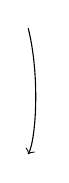
\begin{tikzpicture}\draw[->] (0,1.6) .. controls (.15,1) and (.1,.2) .. (0,0);\end{tikzpicture}}
\[
 \widetilde b=\widetilde b_1\widetilde b_2=b_1b_2
\]
\diagram{\begin{tikzcd}[row sep=huge]
\mathcal E_{(p_1,q_1)(p_2,q_2)}\deleted{\unsure{\simeq}}=M_1\otimes M_2\oplus L_1\otimes L_2\arrow[d,leftrightarrow,"\sim"',"T_{v_{(p_1,q_1)(p_2,q_2)}}"]\\
\mathcal E_{(\widetilde p_1,\widetilde q_1)(\widetilde p_2,\widetilde q_2)}=M_1\otimes M_2\oplus L_1\otimes L_2
\end{tikzcd}}
\margin{$\chi$-scindage défini (comme $q$) par
\diagram{\begin{tikzcd}[column sep=large]
M_1\otimes M_2\arrow[r,no head,"b=b_1b_2"]&L_1\otimes L_2
\end{tikzcd}}}
\margin{$\chi$ sc. défini (comme $\unsure{p.}$) par $-b$}
\inserted{$(=(\eta,\zeta)\longmapsto\eta,\zeta\unsure{+|-}v(\eta))$}
$T_v$ \deleted{\unsure{tr}}ansforme le $\chi$-scindage défini par $b$ en le $\unsure{\varphi|\chi}$-scindage défini par $b+\chi v$.
\deleted{\unsure{Si}} L'on veut que
\[
 b+\chi v=\underset{-b}{\underset{\Vert}{\widetilde b}}\deleted{\unsure{=}}\quad\text{i.e.}\quad v\overset{!}{=}-\frac{2}{\chi}b
\]
Supposons que $\exists\unsure{\gamma}\in k$, tq. $\gamma\chi=2$, \unsure{on peut} prendre \deleted{$\unsure{v}$}
\[
 \boxed{v=-\gamma b}
\]
\mspage{127}

\scanpage{129}
\mspage{128}
\mspage{467}
$({}^{106}1)$ (3 octobre) Ni moi, ni Deligne n'avons jamais eu le moindre doute que les
conjectures de Weil puissent ne pas être valables, et je ne me rappelle pas \unsure{avoi|avoir}
entendu quiconque exprimer de tels doutes. Qualifier le ``résultat'' (i.e. la dé-\newline
monstration de ces conjectures) comme ``surprenant'', témoigne encore du propos
délibéré d'épater la galerie. D'ailleurs à aucun moment depuis l'introduction
de la ``topologie'' et de la cohomologie étales, je n'ai eu le sentiment que ces
conjectures étaient hors d'atteinte, mais plutôt \inserted{(}à partir de 1963\inserted{)} qu'elles ne
manqueraient pas d'être démontrées dans les toutes prochaines années. Au moment
de mon départ, en 1970, je n'avais guère de doute que Deligne, qui était le \unsure{mie|mieux}
placé de tous pour cela, ne tarderait pas à les prouver (ce qu'il n'a pas manqué
de faire), en même temps que les``conjectures standard sur les cycles algébriques
plus fortes, (qu'il s'est par contre attaché à discréditer).

C'est d'ailleurs avec raison que Deligne émet des réserves sur la validité
de ces dernières conjectures, dont je ne suis pas plus convaincu que lui. Mais
la portée d'une conjecture ne dépend pas du fait si elle finira par se révéler
vrai\inserted{e}, ou fausse, pas plus que son caractère de soi-disante ``difficulté'', qui la
rendrait``hors de portée'' - caractère entièrement subjectif, lui. Elle dépend \unsure{un|uni-}\newline
quement du fait si la\quad q u e s t i o n\quad sur laquelle la conjecture met le \unsure{doig|doigt}
(et qui n'avait pas été perçue, avant qu'elle ne soit posée) - si cette \unsure{questio|question}
touche à quelque chose de vraiment essentiel pour notre connaissance des choses.
Or il est evident (pour moi tout au moins!) qu'il ne saurait être question d'\unsure{avo|avoir}
une bonne compréhension des cycles algébriques, ni des propriétés dites ``\unsure{arithme|arithmé-}\newline
tiques'' de la cohomologie des variétés algébriques (ou encore, de la ``géométrie
des motifs''), aussi longtemps que la question de la validité de ces conjectures
n'est pas réglée. Aujourd'hui encore comme lors du Congrès de Bombay en 1968,
je considère cette question, avec celle de la résolution des singularités, \unsure{comme}
l'une des deux questions les plus fondamentales qui se posent en géométrie algé-\newline
brique. Je sens bien la portée de l'une et de l'autre! Cette fécondité \unsure{potentie|potentiel-}\newline
le ne pourra manquer de se manifester, dès l'instant où on ne se bornera plus à
contourner cahin-caha une conjecture décrétée ``trop difficile'', et où quelqu'un
prendra la peine enfin de retrousser ses manches et de s'y coltiner!

\scanpage{130}
\diagram{\begin{tikzcd}[column sep=small]
0\arrow[r,no head]&L_i\arrow[r,no head]&E_i\arrow[r,no head]&M_i\arrow[r,no head]&0
\end{tikzcd}}
, et
\diagram{\begin{tikzcd}[column sep=small]
\pi_i:E_i\arrow[r,no head]&L_i
\end{tikzcd}}
$\chi$-scindage \unsure{donné}
\[
 p=(p_1,p_2)
\]
\diagram{\begin{tikzcd}[column sep=small]
p_i:E_i\arrow[r,no head]&L_i
\end{tikzcd}}
scindage
\[
 \Theta_{p_i}:E_i\simeq M_i\oplus L_i
\]
\diagram{\begin{tikzcd}[column sep=small]
b_i:\pi_i-\chi p_i:M_i\arrow[r]&L_i
\end{tikzcd}}
\diagram{\begin{tikzcd}[column sep=large]
b=b_1\otimes b_2:M_1\otimes M_2\arrow[r,no head]&L_1\otimes L_2
\end{tikzcd}}
d'où $\chi$-trivialisation \unsure{comp.} avec $\pi_{(p_1,p_2)}$,
\diagram{\begin{tikzcd}[column sep=huge]
\mathcal E_{(p_1,p_2)}\deleted{\unsure{\simeq 0}}=(M_1\otimes M_2)\oplus(L_1\otimes L_2)\arrow[r,"\deleted{\unsure{T_{-U}}}","{\Theta_{p,p'}\ \deleted{\unsure{\Theta_{p,p'}}}=T_{-U}}"']&\mathcal E_{p'_1,p'_2}
\end{tikzcd}}
\[
 \pi_{(p_1,p_2)}-\chi\unsure{p|\rho}=b_1\otimes b_2
\]
\[
 \pi_{p_1,p_2}:(\eta,\zeta)\mathbin{\text{---}}\deleted{\unsure{\eta}}\chi\zeta+b_1\otimes b_2(\eta))
\]
\figure{\begin{tikzpicture}\draw (0,0)--(0,4.8);\end{tikzpicture}}
\[
 p'_i=p_i-U_i,\quad U_i:M_i\longrightarrow L_i
\]
\[
 p'=(p'_1,p'_2)
\]
d'où $b'_1,b'_2$, avec
\[
 \unsure{b'_1}=\unsure{b_1}+\chi U_1,\quad b'_2=b_2+\chi U_2
\]
\[
 U=b_1\otimes U_2+U_1\otimes b_2+\chi U_1\otimes U_2
\]
\[
 (\eta,\zeta)\longmapsto(\eta,\zeta\unsure{+|-}U\eta)
\]
\figure{\begin{tikzpicture}\draw (0,0)--(0,.65);\end{tikzpicture}}
\uline{NB} $\Theta_{p,p'}$ transforme $\pi_{(p_1,p_2)}$
\[
 \begin{aligned}
 \pi_{p'_1,p'_2}:\ (\eta,\zeta)&\longmapsto\deleted{\unsure{\eta}}\chi\zeta+(b'_1\otimes b'_2)(\eta)\\
 &=\pi_{(p_1,p_2)}(\eta,\zeta)+U(\eta)
 \end{aligned}
\]
\mspage{129}

\scanpage{131}
\mspage{468}
$({}^{107})$ (4 octobre) J'ai eu occasion déjà de faire mention d'un aspect important
de ces premières cinq années de ma vie, comme d'un``privilège'' de grand prix (*):
une identification profonde et sans problèmes avec mon père, laquelle n'a jamais
été touchée par la peur ou par l'envie. Je me suis rendu compte de cette \unsure{circons|circons-}\newline
tance, et de l'existence même, comme de la silencieuse force, de cette identifi-\newline
cation à mon père, il y a quatre ans seulement (au cours de la méditation sur
mon enfance et sur ma vie qui a suivi celle d'août 79 à mars 80 sur mes parents)
Cette identification était comme le coeur paisible et puissant d'une identifi-\newline
cation à la famille que nous formions, mes parents, ma soeur (qui était mon \unsure{aîné|aînée}
de quatre ans) et moi. Je vouais une admiration et un amour sans limites à mon
père comme à ma mère. Leur personne était pour moi la mesure de toutes choses.

Cela ne signifie nullement que mon attitude à leur égard était celle \unsure{d'une}
approbation automatique, d'une admiration béate. Je ne savais sans doute pas
qu'ils étaient la mesure de toute chose pour moi, mais je savais fort bien \unsure{qu'il|qu'ils}
étaient faillibles comme moi, et il n'y avait en moi aucune crainte qui m'aurait
empêché de constater un désaccord et de le manifester clairement. Dans les
conflits qui m'entouraient\unsure{;|,} je ne craignais pas de prendre partie à ma façon. Ce
ne touchait en rien à une certaine foi, à une assurance qui formaient l'assise
profonde, inébranlable de mon être - plutôt, cela découlait spontanément de \unsure{cett|cette}
foi, de cette assurance même.

Il arrivait que mon père, dans des accès de colère impuissante alors que
ma soeur (sans en avoir l'air) prenait plaisir à le provoquer, la frappe avec
brutalité - et à chaque fois j'en étais outragé, dans un élan de solidarité sans
réserves avec ma soeur. C'étaient là je crois les seuls gros nuages qui \unsure{passaien|passaient}
dans ma relation à\unsure{:}mon père (il n'y en avait pas avec ma mère). Ce n'est pas que
j'approuvais les tours parfois pendables de ma soeur, pas plus je crois qu'ils
ne me troublaient vraiment - ce n'était pas\quad e l l e\quad qui était pour moi la
mesure des choses. Ses tours (dont la raison sûrement m'échappait tout autant
qu'à mon père, qui ``marchait'' à tous les coups, ou à ma mère qui n'avait garde
d'intervenir ni avant ni après) - ces tours en un sens ne tiraient pas vraiment
à conséquence pour moi. C'était ma soeur, elle était comme elle était, voilà \unsure{tou|tout.}
Mais que\quad m o n\quad p è r e\quad se laisse aller à une telle brutalité aveugle\ldots

Les trois êtres les plus proches, qui ensemble ont constitué comme la ma-\newline
trice de mes premières années, étaient déchirés par le conflit, opposant chacun

\figure{\begin{tikzpicture}\draw (0,0)--(3.3,0);\end{tikzpicture}}
(*) Voir la note ``\unsure{Le.massacre|Le massacre}'', n° 87.
\mspage{130}

\scanpage{132}
\[
\deleted{\Theta_{p+U}(x)=}\qquad
\Theta_p(x)=\deleted{\unsure{p(x)|\psi(x)}}\psi(x)\oplus p(x)
\]
\[
\Theta_{p+U}(x):\quad\psi(x)\oplus(p(x)+U\psi(x))
\qquad\boxed{b_i=(\pi_i-\chi p_i)}
\]
\diagram{\begin{tikzcd}[column sep=huge,row sep=large]
& E_1\vee E_2\arrow[dl,"\Theta_{p_1,p_2}"',"\sim"]\arrow[d,no head,"\Theta_{p'_1,p'_2}"',"\sim"]\arrow[dr,"\Theta_{p''_1,\unsure{p''_3|p''_2}}","\sim"'] &\\
M\oplus L\arrow[r,"\substack{(U_1,U_2,U)\\\Theta_{(p_1,p_2)(p'_1,p'_2)}\\\sim}"]\arrow[rr,bend right=25,"\substack{U''_1,U''_2,U''\\\Theta_{(p_1,p_2)(p''_1,p''_2)}}"'] & M\oplus L\arrow[r,"\substack{(U'_1,U'_2,U')\\\Theta_{(p'_1,p'_2)(p''_1,\unsure{p''_3|p''_2})}\\\sim}"] & M\oplus L
\end{tikzcd}}
\[
(\eta,\zeta)\longmapsto(\eta,\zeta-U\eta)
\qquad(\eta,\zeta)\longmapsto(\eta,\zeta-U'\eta)
\]
\[
\operatorname{Hom}(M_i,L_i)\quad
\operatorname{Hom}(M_i,L_i)\quad\operatorname{Hom}(M_i,L_i)
\]
\[
\begin{array}{ccc}
\downarrow&\downarrow&\\
b_i&b'_i=b_i+\chi U_i&b''_i=b'_i-\chi U'_i
\end{array}
\qquad(\eta,\zeta)\longrightarrow(\eta,\zeta+
\]
\[
b_1\otimes b_2\in\operatorname{Hom}(M,L)
\qquad
\begin{aligned}
b'_1\otimes b'_2&=(b_1-\chi U_1)\otimes(b_2-\chi U_2)\\
&=b_1b_2\unsure{+|-}\chi U
\end{aligned}
\]
\[
(\pi-\chi\,p_1*p_2)^{\Theta_{p_1,p_2}}
\]
\[
\left\{\begin{aligned}
p'_1*p'_2&=p_1*p_2-U\\
p''_1*p''_2&=p'_1*p'_2-U'=p_1*p_2-U''\\
&\Longrightarrow U''=U+U'
\end{aligned}\right.
\]
\[
b''_1\otimes b''_2=b'_1\otimes b'_2-\chi U'
=b_1\otimes b_2-\chi\underbrace{(U+U')}_{U''}
\]
\margin{\diagram{\begin{tikzcd}[row sep=small]
(p_1,p_2)\arrow[d]\\(p'_1,p'_2)\arrow[d]\\\uline{(p''_1,p''_2)}
\end{tikzcd}}
\((p_1,p_2)\quad(p''_1,p''_2)\)}
\[
\left\{\begin{aligned}
U&=b_1\otimes U_2+U_1\otimes b_2+\chi U_1\otimes U_2\\
U'&=b'_1\otimes U'_2+U'_1\otimes b'_2+\chi U'_1\otimes U'_2\\
U''&=b_1\otimes U''_2+U''_1\otimes b_2+\chi U''_1\otimes U''_2
\end{aligned}\right.
\]
(où \(U''_1=U_1+U'_1,\quad U''_2=\unsure{U_2|U'_2}+U'_2\))
\[
\underbrace{b_1,b_2;\ U_1,U_2}_{\downarrow}\qquad
\underbrace{U'_1,U'_2}_{|}
\]
\[
\left\{\begin{aligned}
b'_1&=b_1+\chi U_1,\quad b'_2=b_2+\chi U_2\quad\deleted{(b'_1,b'_2)}\\
b''_1&=b'_1+\chi U'_1,\quad b''_2=b_2+\chi U'_2
\end{aligned}\right.
\]
\[
\deleted{\unsure{U|b}=}\qquad
\deleted{=(b_1-\chi U_1)\otimes U'_1+U'_2\otimes(b_2-\chi U'_2)+\chi U'_1\otimes\unsure{b_2|U'_2}}
\]
\margin{\figure{\begin{tikzpicture}\draw[<->](0,0)--(0,2.5);\end{tikzpicture}}
\(\begin{aligned}b&=b_1\otimes b_2\\b'&=b'_1\otimes b'_2\\b''&=b''_1\otimes b''_2\end{aligned}\)}
\uline{1°)} Je dis que \(U''=U+U'\),
\[
\deleted{b''_1=b'_1+\chi U''_1,\quad b''_2=}\qquad\deleted{\unsure{b|U}=}
\]
\[
\begin{aligned}
U''&=b_1\otimes(U_2+U'_2)+(\unsure{U_1|U''_1}+U'_1)\otimes b_2
+\chi\underbrace{(U_1+U'_1)\otimes(U_2+U'_2)}\\
&=U+b_1\otimes U'_2+\underbrace{U'_1\otimes b_2+\chi U'_1\otimes U_2}_{U'_1\otimes(b_2+\chi U_2)}
+\chi U_1\otimes U'_2+\chi U'_1\otimes U'_2\\
&\hspace{3em}{}+(b_1+\chi U_1)\otimes U'_2+\chi U'_1\otimes U'_2
\end{aligned}
\qquad=\deleted{\unsure{U|b}}
\]
\mspage{131}

\scanpage{133}
\mspage{469}
d'eux et à lui-même, et aux deux autres: conflit insidieux,au visage impassible
entre ma mère et ma soeur, et \unsure{conflit} aux violents éclats entre mon père et ma
mère d'un côté, ma soeur de l'autre, qui chacune pour son propre compte (et sans
que personne du vivant de mes parents ait jamais fait mine de s'en apercevoir...
le faisait marcher à sa façon. La chose mystérieuse, extraordinaire, c'est \unsure{qu'en|qu'en-}\newline
touré ainsi par le conflit en ces années les plus sensibles, les plus cruciales
de la vie, celui-ci soit resté\quad e x t é r i e u r\quad à moi, qu'il n'ait pas \unsure{vrai|vrai-}\newline
ment ``mordu'' sur mon être en ces années-là et ne s'y soit installé à demeure.

La division dans mon être, qui a marqué ma vie tout autant que celle de \unsure{to|tout}
autre, ne s'est pas installée en moi en ces années, mais en les deux ou trois \unsure{an|ans}
qui ont suivi, de ma sixième à ma huitième année environ. A un certain moment
(que j'ai cru pouvoir situer à quelques mois près, et qui se placerait dans ma
huitième année) il y a eu un certain\quad b a s c u l e m e n t\quad, au bout de plus
de deux ans de séparation avec mes parents (qui ne se souciaient guère de me
donner signe de vie) et de ma soeur. C'était avant tout une\quad r u p t u r e\quad
a v e c\quad m o n\quad e n f a n c e\quad, ``enterrée'' à partir de ce moment par d'effica-\newline
ces mécanismes d'oubli (qui sont restés en place, à peu de choses près, jusqu'à
aujourd'hui même). A un certain niveau profond (pas le plus profond pourtant...)
mes parents ont alors été déclarés par moi comme des ``étrangers'', tout comme mon
enfance était désormais déclarée ``étrangère''. J'ai a b\unsure{.}d i q u é\quad, en un sens:
pour être accepté dans le monde qui m'entourait désormais, j'ai décidé d'être
comme ``eux'', comme les adultes qui y font la loi - d'acquérir et de développer
les armes qui y forcent le respect, de me battre à armes égales dans un monde où
seule, une certaine espèce de ``force'' est acceptée et prisée...

C'était d'ailleurs cette force-là aussi qui avait la préférence de mes pa-\newline
rents, lesquels avaient entouré mes premières années. Et là je reviens à cette
``chose mystérieuse'' (dont je viens de m'éloigner, en suivant le fil d'une autre
association suscitée par cette chose), l' a b s e n c e\quad d e\quad d i v i s i o n\quad
e n\quad m o i\quad, en ces premières années de ma vie.

Peut-être le mystère n'est plus pour moi en cette absence, mais plutôt en \unsure{;}
ceci: que mes parents, mon père comme ma mère, m'aient chacun alors \unsure{a c c e p t|a c c e p t é}
d a n s\quad m a\quad t o t a l i t é\quad, et totalement: dans ce qui en moi est ``viril''
est \unsure{.}``homme'', et dans ce qui est ``femme''. Ou pour le dire autrement: que mes pa-\newline
rents, déchirés l'un et l'autre par le conflit, reniant chacun une partie essen-\newline
tielle de leur être - incapable chacun d'une ouverture aimante à lui-même et à
l'autre, comme d'une ouverture aimante à ma soeur... que néanmoins ils aient
trouvé une telle ouverture, une acceptation sans réserve, vis à vis de moi
\mspage{132}

\scanpage{134}
\diagram{\begin{tikzcd}[column sep=huge,row sep=large]
& E_1\unsure{\wedge|\vee}E_2\arrow[dl,very thick,"\Theta_{p_1*p_2}"']\arrow[dr,"\Theta_{p'_1*p'_2}=\Theta_{p_1*p_2}\unsure{-|+}U"] &\\
(M_1\otimes M_2)\oplus(L_1\otimes L_2)\arrow[rr] && (M_1\otimes M_2)\oplus(L_1\otimes L_2)\\
b_1,b_2&&b'_1,b'_2
\end{tikzcd}}
\[
\unsure{T_U|\Lambda_U}:(\unsure{\eta|\zeta},\unsure{\zeta|\xi})\longmapsto(\eta,\zeta+U(\eta))
\]
\[
U=b_1(p_1)\otimes U_2+U_1\otimes b_2(p_2)+\chi U_1\otimes U_2
\]
\[
b'_1=b_1-\chi U_1,\qquad b'_2=b_2-\chi U_2
\]
\[
p'_1=p_1\unsure{+|-}U_1\psi_1,\quad
\unsure{p'_i|p'_2}=p_2\unsure{+|-}U_2\psi_2
\]
\diagram{\begin{tikzcd}[row sep=small]
U_1:M_1\arrow[r]&L_1\\
U_2:M_2\arrow[r,no head]&\unsure{L_2|L_1}
\end{tikzcd}}
\[
p'_1*p'_2=p_1*p_2\unsure{+|-}
\left[\underbrace{(\pi_1-\chi p_1)}_{b_1(p_1)}\otimes U_2
+U_1\otimes\underbrace{(\pi_2-\chi p_2)}_{b_2(p_2)}\right]
\deleted{\unsure{+}}-\chi U_1\otimes U_2
\]
\deleted{\(\unsure{b_2|b_1}\)}
\margin{\figure{\begin{tikzpicture}\draw[->](0,0)--(.25,.45);\end{tikzpicture}}
signe étrange\\
\unsure{qui doit|qui où le} \unsure{pourtant être|produit être}\\
\deleted{\unsure{étrange}}}
\[
U_1*U_2=-\chi U_1\otimes U_2
\]
Ces signes sont \unsure{dûs} au signe \(\underset{\mathcal E}{-\mathrm{id}}\) dans le diag. \unsure{non}
commutatif. (pour une extension de \(\underline O\) par \(\mathcal H\)
\diagram{\begin{tikzcd}[column sep=large,row sep=large]
0\arrow[r,no head]&\mathcal H\arrow[r,no head,"\alpha"]\arrow[d,"-\mathrm{id}"']&\mathcal E\arrow[r,no head,"\psi"]\arrow[d,"\Phi"',"\unsure{R|\sim}"]&\underline O\arrow[r]\arrow[d,equal]&0\\
0\arrow[r,no head]&\mathcal H\arrow[r]\arrow[d,equal]&\operatorname{Hom}^{!}(E,\mathcal H)\arrow[r]&O\arrow[r,no head]&0\\
&\operatorname{Hom}(\underline O,\mathcal H)&&&
\end{tikzcd}}
\[
\varphi(x,y)=-x\psi(y)+y\psi(x)
\]
\figure{\begin{tikzpicture}\draw[->](.3,.3)--(0,0);\draw(.15,.03)--(.35,.03);\end{tikzpicture}}
\[
\deleted{=\unsure{\lambda\operatorname{Hom}|\lambda}\ \mathcal E\longrightarrow\mathcal H}
\qquad f\longmapsto\lambda
\]
\deleted{\unsure{qui a le}\ \unsure{val.}}\ \(\exists\lambda;\)
\[
=\left\{f:\mathcal E\mathrel{-\!\!-\!\!-}\mathcal H\ \middle|\ 
f\circ\alpha=\unsure{\alpha|a}(\lambda\,\mathrm{id}_{\mathcal H}\right\}
\]
\margin{\diagram{\begin{tikzcd}[column sep=small,row sep=small]
&\arrow[r,mapsto]&\deleted{\unsure{\eta}}\\
\zeta_1,\eta_1\arrow[rr]&&\chi\eta_1+b_1(\zeta_1)\\
M_1\otimes M_2\arrow[u]&L_1\otimes L_2\arrow[ul]&
\end{tikzcd}}}
Si on pose
\[
p'_1=p_1-U'_1,\quad p'_2=p_2-U'_2,\quad
p'_1*p'_2=p_1*p_2-U'
\]
\[
\text{d'où }\left\{\begin{aligned}
U'_1&=-U_1\\
U'_2&=-U_2\\
\unsure{U'|U'_0}&=-U
\end{aligned}\right.
\quad\unsure{\sim}\quad
U'=-b_1\otimes U_2-U_1\otimes b_2+\chi U_1\otimes U_2
\]
\[
\boxed{U'=b_1\otimes U'_2+U'_1\otimes b_2+\chi U'_1\otimes U'_2}
\]
\margin{\unsure{soit|c'est} la formule \unsure{trouvée}....}
\mspage{133}

\scanpage{135}\mspage{470}
leur fils.

Pour le dire autrement encore: à aucun moment en ces premières cinq années
de ma vie, je n'ai connu le sentiment de\quad h o n t e\quad d'\quad ê t r e\quad c e\quad q u e\quad
j e\quad s u i s\quad, que ce soit dans mon corps et ses fonctions, ou dans mes \unsure{pulsion|pulsions}
mes penchants,\unsure{.}mes actions. A aucun moment je n'ai eu à renier quelque chose en
moi, pour être accepté par mon entourage et pouvoir vivre en paix avec lui.

Il arrivait bien sûr que je fasse des choses qui ne ``passaient'' pas: comme
tous les enfants il m'arrivait sûrement d'être pénible, voire insupportable
quand je m'y \unsure{méttais|mettais} - et il était clair parfois qu'il me fallait rectifier le
tir. Je ne faisais pas la loi, ni n'étais tenté de vouloir la faire, n'ayant pas
à compenser quelque mutilation secrète. Et dans l'amour de mes parents pour moi,
il n'aurait pu y avoir de place pour l'adulation, la complaisance aux caprices -
pour une approbation \unsure{inconditionnelle}. Mais s'il arrivait forcément que je me
fasse ``envoyer sur les \unsure{roses|coses}'' par mon père ou par ma mère (tout comme l'inverse
pouvait parfois se produire), jamais dans ces années-là l'un ni l'autre ne m'ont
fait honte, d'un acte ou d'un comportement qui n'aurait pas eu l'heur de leur
plaire.

Sur le fond d'une identification profonde au père, sans \unsure{ambiguité|ambiguïté} aucune,
ma personne comme enfant m'apparaît aujourd'hui comme empreinte à la fois de vi-\newline
rilité et de féminité, fortes l'une comme l'autre.

Il me semble qu'en chaque être et en chaque chose, dans ces indissolubles
et fluctuantes épousailles des qualités yin et yang en lui qui font de lui ce
qu'il est, et dont le délicat équilibre est la beauté profonde, l'harmonie qui
vit en cet être ou en cette chose - que dans cette union intime du yin et du
yang il y a souvent (peut-être toujours) une note de fond, une ``dominante'',
qui est soit yin, soit yang. Cette note de fond n'est pas toujours aisée à dé-\newline
celer en une personne, à cause des mécanismes de répression plus ou moins effi-\newline
caces et complets, qui faussent le jeu en substituant, à une harmonie originelle
une image d'emprunt. Ainsi mon ``image de marque'' pendant quarante ans a été une
image presque exclusivement virile - sans d'ailleurs jamais se voir mettre en
cause ni même être décelée comme telle, par moi-même ni (il me semble) par au-\newline
trui, jusqu'à ma quarante-huitième année. J'ai tendance à croire pourtant que
la note de fond présente à la naissance reste présente pendant la vie entière,
dans des couches profondes tout au moins qui jamais peut-être ne trouveront
l'occasion de se manifester au grand jour. Dans mon propre cas, chose étrange, \unsure{j|je}
ne saurais aujourd'hui encore dire quelle est cette note dominante, celle donc
\mspage{134}

\scanpage{136}
\diagram{\begin{tikzcd}[column sep=small,row sep=large]
0\arrow[r]&L\arrow[r,no head]\arrow[d,"-\mathrm{id}_L"']&E\arrow[r,"\psi"]\arrow[d,"\sim"]&\underline O\arrow[r]\arrow[d,equal]&0\\
\arrow[r,no head]&L\arrow[r]&\operatorname{Hom}^{!}(E,L)\arrow[r,no head]&\underline O\arrow[r,no head]&0
\end{tikzcd}}
\[
\unsure{x}\longmapsto
\left[y\longmapsto(-x\psi(y)+y\psi(x))\right]
\]
\diagram{\begin{tikzcd}E\arrow[r,"\psi(x)"']&L\end{tikzcd}}
\[
{}_{\lambda_1}E_1*{}_{\lambda_2}E_2\simeq
\]
\figure{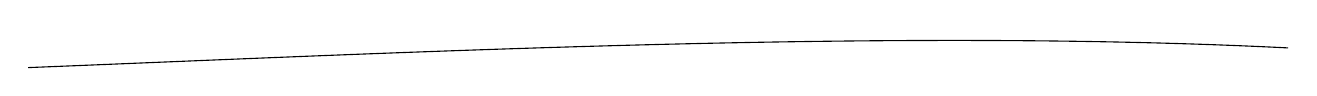
\begin{tikzpicture}\draw(0,0)..controls(5,.2)and(11,.5)..(16,.25);\end{tikzpicture}}
\[
\left|\begin{aligned}
(f_1*f_2)(x_1*x_2)&=\unsure{\Psi_1(f_1)[|[\Psi_1(f_1)}
\pi_1(x_1)\otimes f_2(x_2)+f_1(x_1)\otimes
\unsure{\Psi_2 f_2|\Psi_2(f_2)}\pi_2(x_2)-\chi f_1(x_1)\otimes f_2(x_2)]\\
(f_1*f_2)(u_1\otimes u_2)&=\lambda_1\lambda_2\,u_1\otimes u_2
\end{aligned}\right.
\]
\figure{\begin{tikzpicture}\draw(0,0)..controls(6,.5)and(11,.7)..(16,.5);\end{tikzpicture}}
\[
(f_1*U_2)(x_1*x_2)=\Psi_1(f_1)\pi_1(x_1)\otimes
\underbrace{\unsure{U_2|f_2}(x_2)}_{U_2(\psi_2(x_2))}
-\chi f_1(x_1)\otimes\unsure{U_2|f_2}(x_2)
\]
\deleted{\((U_1*f_2)(x_1*x_2)\)}
i.e.
\[
(f_1*U_2)(x_1*x_2)=
\underbrace{\bigl(\Psi_1(f_1)\pi_1-\overset{\Psi_1(\pi_1)}{\overset{\Vert}{\chi}}f_1\bigr)}_{\text{nul sur }L_1}
\otimes U_2\,(x_1\otimes x_2)
\]
\[
\bigl([\pi'_1,f'_1]'\otimes U_2\bigr)(x_1\otimes x_2).
\]
de \(=\)
\[
\left\{\begin{aligned}
U_1*f_2\,(x_1*x_2)&=
\bigl(U_1\otimes[\pi'_2,f'_2]'\bigr)(x_1\otimes x_2)\\
(U_1*U_2)(x_1*x_2)&=-\chi\cdot U_1(x_1)\otimes U_2(x_2)=
\end{aligned}\right.
\]
\margin{\figure{\begin{tikzpicture}\draw[->](0,0)--(.15,.5);\end{tikzpicture}}
signe étrange!}
\figure{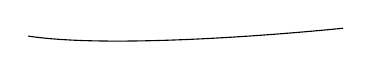
\begin{tikzpicture}\draw(0,0)..controls(1,-.15)and(3,0)..(4,.1);\end{tikzpicture}}
\[
(\unsure{x_1|u_1}+u_1)*(\unsure{x_2|u_2}+u_2)
=x_1*x_2+\underbrace{x_1*u_2}_{\underbrace{\pi_1(x_1)}_{b_1}\otimes u_2}
+\underbrace{u_1*x_2}_{u_1\otimes\underbrace{\pi_2(x_2)}_{b_2}}
+\underbrace{u_1*u_2}_{\Vert\ \chi u_1\otimes u_2}
\]
\mspage{135}

\scanpage{137}\mspage{471}
qui a imprégné ma première enfance et qui était ``mienne'' déjà à ma naissance.
Divers signes m'ont fait soupçonner plus d'une fois que cette note est ``yin'',
que ce sont les qualités ``féminines'' qui dominent dans mon être, quand celui-ci
trouve occasion de se manifester spontanément, en les instants où il est libre
des conditionnements de toutes sortes qui se sont accumulés en moi depuis l'en-\newline
fance. Pour le dire autrement: il se pourrait que ce qui est force créatrice en
mon corps et en mon esprit, ce que j'ai appelé parfois ``l'enfant'' ou ``l'ouvrier''
en moi (par opposition au ``patron'' qui représente la structure du moi, c'est à
dire ce qui est conditionné en moi, la somme ou le résultat du conditionnement
accumulé en ma personne) - que cette force soit plus ``féminine'' encore que
``virile'' (alors que par nature et nécessité elle est l'un, et l'autre).

Ce n'est pas le lieu ici de passer en revue tous ces ``signes''. La chose
importante d'ailleurs n'est\quad p a s\quad si cette note dominante profonde en moi
est ``féminine'', ou si elle est ``virile''. C'est plutôt, que je sache en chaque
instant\quad ê t r e\quad m o i - m ê m e\quad, en accueillant sans réticence aussi bien
les traits et les pulsions en moi par lesquels je\unsure{:} suis ``femme'', que ceux par
lesquels je suis ``homme'', et en leur permettant de s'exprimer librement.

Quand j'étais enfant, dans ces premières années, il n'était pas rare que \unsure{de|des}
personnes étrangères me prennent pour une fille - sans d'ailleurs que la chose
crée jamais en moi le moindre malaise, le moindre sentiment d'insécurité. \unsure{C'étai|C'était}
surtout ma voix je crois qui faisait cet effet, une voix très claire, aigüe -
sans compter que j'avais de longs cheveux (le plus souvent ébouriffés), \unsure{peut-êtr|peut-être}
simplement parce que ma mère (qui ne manquait pas d'autres soucis) ne prenait \unsure{pas}
souvent le loisir de me les couper tant soit peu. J'étais par ailleurs fort \unsure{comme}
un turc et les jeux un peu violents ou casse-cou ne me déplaisaient pas, ce qui
n'empêchait nullement un penchant pour le silence, voire même pour la solitude,
et un penchant également pour jouer à la poupée (*). Je n'ai pas souvenir que
quelqu'un se soit moqué de moi à ce propos, mais la chose sûrement n'a guère pu
manquer de se produire ici et là. Si de tels incidents ont passé sans laisser
trace de blessure ou d'humiliation, c'est sûrement qu'ils ne recueillaient aucun
écho ou amplification, par quelque sentiment d'insécurité en moi, alors que
l'acceptation de celui que j'étais, par ceux qui seuls pour moi comptaient vrai-\newline
ment, était au delà de toute question. La moquerie n'aurait pu m'atteindre,
elle ne pouvait que se retourner contre celui qui devait m'apparaître comme bien
sot, pour faire mine de trouver à redire à la chose la plus naturelle du monde.

\figure{\begin{tikzpicture}\draw(0,0)--(3,0);\end{tikzpicture}}
(*) Si ce penchant paraît rare chez les petits garçons, c'est surtout je crois
parce qu'il est systématiquement découragé par l'entourage.
\mspage{136}

\scanpage{138}
\deleted{\((f_1*f_2)(x_1*x_2)=\)}
\[
(f_1*f_2)\big|_{E_1\otimes E_2}:\quad E_1\otimes E_2\mathrel{-\!\!-\!\!-}L_1\otimes L_2
\]
\[
\boxed{\begin{aligned}
f_1*f_2\,(x_1*x_2)&=\lambda_1\pi_1(x_1)\otimes f_2(x_2)
+f_1(x_1)\otimes\lambda_2\pi_2(\overset{\deleted{\unsure{\lambda_2+}}}{x_2})
-\chi f_1(x_1)\otimes f_2(x_2)\\
\text{i.e. }\quad f_1*f_2\big|_{E_1\otimes\unsure{E_1|E_2}}
\quad[E_1\otimes E_2\mathrel{-\!\!-\!\!-}L_1\otimes L_2]
&\overset{!}{=}\lambda_1\pi_1\otimes f_2+f_1\otimes\lambda_2\pi_2-\chi f_1\otimes f_2
\end{aligned}}
\]
\[
f_1*f_2\,(u_1\otimes u_2)=\lambda_1\lambda_2(u_1\otimes u_2)
\]
\deleted{\unsure{Si on}}
Vérifions
\[
f_1*f_2\,(x_1*u_2)=\lambda_1\lambda_2\pi_1(x_1)\otimes u_2
\]
\[
\lambda_1\pi_1(x_1)\unsure{)}\otimes\lambda_2u_2+
\deleted{f_1(x_1)\otimes\underbrace{\lambda_2\chi}u_2}
-\deleted{\underbrace{\chi f_1(x_1)\otimes\lambda_2u_2}}
\qquad OK
\]
\[
\begin{aligned}
(\pi_1*\pi_2)(x_1*x_2)&=\chi\{\pi_1(x_1)\otimes\pi_2(x_2),\\
(\pi_1*\pi_2)(u_1\otimes u_2)&=\chi^2\unsure{u_1}\otimes u_2
\end{aligned}\quad\Big]
\qquad\frac1\chi\,\pi_1*\pi_2=\pi
\]
\[
x_1*x_2\simeq\unsure{\Psi_1(x_1)|\psi_1(x_1)}
\]
\figure{\begin{tikzpicture}\draw(0,0)--(0,1.8);\end{tikzpicture}}
\[
\begin{array}{cc}
L_i&p_i\\[1em]M_i&q_i
\end{array}
\qquad1+\underbrace{p_1q_1},\quad1+\underbrace{p_2q_2}
\qquad1+(p_1p_2)(q_1q_2)
\]
\[
\deleted{[x,y]=}\qquad
x\longrightarrow\deleted{\unsure{\psi(x)y|y(x)\psi}}
\psi(x)\unsure{T|\pi}-\chi\unsure{x}
\]
\mspage{137}

\scanpage{139}\mspage{472}
Je savais bien d'ailleurs que ce genre de sottise un peu étrange n'est
nullement chose rare, que la seule vue de la nudité peut être cause de scandale!
Pourtant aussi loin que je pouvais me souvenir, j'avais eu l'occasion de voir ma
mère, mon père\quad et ma soeur nus, et toute occasion aussi de satisfaire ma légi-\newline
time curiosité quant à comment chacun d'eux ainsi que moi-même étions faits. Il
était bien évident qu'il n'y avait nulle cause de scandale dans la conformation
des hommes ou des femmes, qui me paraissait décidément très bien comme elle
était - et plus particulièrement (je n'en faisais nullement mystère) celle des
femmes.

\(({}^{108})\) (5 octobre) C'est en 1933, alors que j'étais dans ma sixième année, que se
place le premier tournant crucial dans ma vie, qui a été en même temps un tour-\newline
nant crucial aussi dans la vie de ma mère comme de mon père, dans leur relation
l'un à l'autre comme dans celle à leur enfants. C'est l'épisode de la \unsure{destructio|destruction}
violente et définitive de la famille que nous formions tous les quatre, destruc-\newline
tion dont j'ai été le premier et le seul, quarante-six ans plus tard, à faire le
constat et à suivre les péripéties, dans la correspondance de mes parents et
dans un ou deux souvenirs exsangues, énigmatiques et tenaces, patiemment sondés
et déchiffrés - bien longtemps après la mort de mon père et celle de ma mère (*).

Ce n'est pas mon propos de m'étendre ici sur ce que j'ai appris et compris
au cours de ce long travail, au sujet de la portée et du sens de cet épisode.
J'ai déjà fait allusion il y a trois jours à ce tournant (**), comme marquant la
fin brutale de la première des trois grandes périodes, dans l'histoire des épou-\newline
sailles du yin et du yang en moi. En décembre 1933, je me trouve largué en toute
hâte dans une famille étrangère, que moi, ni ma mère qui m'y amenait depuis
Berlin, n'avions jamais vue. En fait, ces gens inconnus chez qui elle m'amenait
étaient simplement les premiers venus qui veuillent bien de moi comme ``pension-\newline
naire'' pour une pension plus que modique, et avec aucune garantie d'aucune sorte
que celle-ci serait jamais payée, alors que ma mère s'apprêtait à rejoindre au
plus vite mon père, qui se morfondait à l'attendre à Paris. C'était une chose en-

\figure{\begin{tikzpicture}\draw(0,0)--(3,0);\end{tikzpicture}}
(*) Mon père est mort à Auschwitz en 1942, ma mère est morte en 1957. Le travail
dont je parle ici s'est poursuivi entre août 1979 et octobre 1980.

(**) Voir fin de la note ``Yang enterre yin - ou le muscle et la tripe'', n° 106.
\mspage{138}

\scanpage{140}
\diagram{\begin{tikzcd}[row sep=small]
M_1\arrow[d,bend left=35,no head,"q_1"]\\
E_1\arrow[d,"\alpha_1"']\arrow[d,bend left=35,no head,"p_1"]\\L_1
\end{tikzcd}}
\diagram{\begin{tikzcd}[column sep=large,row sep=large]
&&\deleted{M_1\otimes M_2}\\
(E_1\otimes L_2)\oplus(L_1\otimes E_2)\arrow[r]\arrow[dr,"\unsure{\pi|\alpha}"']&
\underset{x_1\otimes x_2}{E_1\otimes E_2}\arrow[dr,"\unsure{\lambda_1|\lambda}"]&
\underset{m_1\otimes m_2}{M_1\otimes M_2}\arrow[l]\arrow[r,no head]&0\\
&L_1\otimes L_2\arrow[r,no head]&
\underset{x_1*x_2}{E}\arrow[r]\arrow[ul,phantom,"\text{comm.}"]\arrow[l,bend left=35,"p"]\arrow[u,bend right=35,"\deleted{\unsure{q}}"]&
\underset{m_1\otimes m_2}{M_1\otimes M_2}\arrow[l,bend left=35,"q"]
\end{tikzcd}}
\[
x_1,x_2\longmapsto m_1\otimes m_2
\qquad q(m_1\otimes m_2)=\unsure{q(m_1)|q_1(m_1)}*\unsure{q(m_2)|q_2(m_2)}
\]
\[
\begin{aligned}
p(\unsure{x_1*x_2|x_1\otimes x_2})
&=x_1*x_2-q(m_1\otimes m_2)\\
&=x_1*x_2-\unsure{q(m_1)|q_1(m_1)}*\unsure{q(m_2)|q_2(m_2)}
\end{aligned}
\]
\[
\unsure{q(m_1)|q_1(m_1)}=x_1-p_1(x_1),\qquad
\unsure{q(m_2)|q_2(m_2)}=x_2-p_2(x_2)
\]
\[
\begin{aligned}
p(x_1*x_2)&=x_1*x_2-(x_1-p_1(x_1))*(x_2-p_2(x_2))\\
&=x_1*p_2(x_2)+p_1(x_1)*x_2-\underbrace{p_1(x_1)*p_2(x_2)}
\end{aligned}
\]
\[
\deleted{=\chi\bigl(x_1\otimes p_2(x_2)+p_1(x_1)\otimes x_2
-\unsure{\chi}p_1(x_1)\otimes p_2(x_2)\bigr)}
\]
\[
u_1*u_2=\chi u_1\otimes u_2,\qquad
p(u_1*u_2)=\chi u_1\otimes u_2
\]
\deleted{\(p(\unsure{x_1})\)}
\[
\boxed{(f_1*f_2)(x_1*x_2)=
\underset{\Vert\ \lambda_1\pi_1(x_1)}{\lambda_1x_1}*f_2(x_2)
+f_1(x_1)*\lambda_2x_2-\chi f_1(x_1)\otimes f_2(x_2)}
\]
\deleted{Si \(x_1,x_2\in L\)}
Si \(x_1\unsure{=|\in}u_1\in L_1,\quad x_2=u_2\in L_2\)
\[
2\lambda_1\unsure{\lambda_2\chi|\chi\lambda_2}x_1\otimes x_2
-\unsure{\chi}\lambda_1\lambda_2x_1\otimes x_2=
\]
\[
\deleted{\lambda-\chi\qquad(2-\chi)\lambda_1\lambda_2u_1\otimes u_2}
\]
\[
2-\chi=1
\]
\[
\begin{aligned}
(f_1*f_2)(u_1\otimes u_2)&:\lambda_1\lambda_2u_1\otimes u_2\\
&=f_1(u_1)\otimes f_2(u_2)
\end{aligned}
\]
\margin{\[
\underbrace{xy-(x-x)(y-y)}_{\Vert\quad xy+yx-xy}=xy
\]
\figure{\begin{tikzpicture}\draw(.7,1.8)--(0,0);\end{tikzpicture}}
\deleted{\(\unsure{f}\)}}
\mspage{139}

\scanpage{141}\mspage{473}
tendue entre mes parents que tout allait être pour le mieux tant pour moi à \unsure{Blan|Blan-}\newline
kenese (près de Hambourg), que pour ma soeur qui depuis quelques mois avait été
larguée à la fin des fins dans une institution à Berlin pour enfants handicapés
(où on avait bien voulu d'elle, bien qu'elle n'était pas plus handicapée que moi
ou nos parents).

En dénouement à six mois étranges, lourds de menace sourde\quad et d'angoisse,
je me suis retrouvé du jour au lendemain dans un monde totalement différent du
seul monde que j'avais connu dans ma vie, celui formé par mes parents et par ma
soeur et moi. Je m'y retrouvais comme un parmi un groupe de pensionnaires, qui
mangions à part de la famille et faisions figure d'enfants de deuxième catégorie
pour les enfants de la maison, lesquels formaient un monde à part et nous regar-\newline
daient de haut. De ma mère je recevais une lettre hâtive et guindée de loin en
loin, et de mon père jamais une ligne de sa main, pendant les cinq ans que j'y
suis resté (jusqu'en 1939, à la veille de la guerre, quand j'ai fini par \unsure{rejoind|rejoindre}
mes parents sous la pression des événements).

Le couple qui m'avait accueilli m'a vite pris en affection. Aussi bien lui
ancien pasteur qui avait quitté le sacerdoce et vivait d'une maigre pension et
de leçons particulières de latin, de grec et de mathématiques, que sa femme pé-\newline
tillante de vie et parfois de malice, étaient des gens peu ordinaires, \unsure{attachant|attachants}
à bien des égards. Lui était un humaniste de vaste culture qui s'était un peu
égaré dans la politique, et avait eu maille à partir avec le régime nazi, qui a
fini par le laisser tranquille. Après la guerre j'ai renoué et je suis resté en
relations suivies avec eux jusqu'à la mort de l'un et de l'autre (*).

De lui et surtout d'elle, tout comme de mes parents, j'ai reçu du meilleur
comme aussi du pire. Aujourd'hui, avec un long recul, je leur suis reconnaissant
(comme je le suis à mes parents) pour ce ``meilleur'', comme aussi pour ce ``pire''.
C'est ce meilleur et ce pire que j'ai reçu, de mes parents d'abord, d'eux \unsure{ensuit|ensuite}
qui a formé le plus gros du volumineux ``paquet'' que j'ai reçu en partage dans \unsure{mo|mon}
enfance (comme chacun reçoit le sien...)\inserted{,}qu'il m'appartenait de déballer et \unsure{d'ex|d'exa-}\newline
miner. Ils font partie de la substance, de la richesse de mon passé, dont il ne
tient qu'à moi de nourrir mon présent.

Mon nouveau milieu était tout ce qu'il y a de ``comme il faut'' et de \unsure{confor|confor-}\newline
miste à beaucoup d'égards, avec en tous cas les attitudes répressives de rigueur
pour tout ce qui concerne le corps et, plus particulièrement, le sexe. Il a \unsure{fall|fallu}

\figure{\begin{tikzpicture}\draw(0,0)--(3,0);\end{tikzpicture}}
(*) Elle est morte à l'âge de 99 ans, il y a deux ans, et j'ai encore pu la voir
morte, en tête à tête avec elle, la veille de l'enterrement.
\mspage{140}

\scanpage{142}

Si on a pu définir $F_{11}$, \unsure{avec} commutativité des deux autres carrés, alors l'hom $F$ est un hom d'ext. au sens strict (avec id sur $L_1\otimes L_2$ et sur $M_1\otimes M_2$), donc c'est un iso.

\unsure{Concentrons} sur $F_{11}:E_1\otimes E_2\unsure{\longrightarrow|\mathrel{-\!\!-\!\!-}}E_1\otimes E_2$ seulement.

1°) Connu sur $E_1\otimes_0 E_2$, et doit \unsure{être} le composé
\[
 E_1\otimes_0 E_2\xrightarrow{\pi}L_1\otimes L_2\mathrel{-\!\!-\!\!-}E_1\otimes E_2
\]
($\chi$-rétraction de $E_1\otimes_0 E_2$ sur le sous-module $L_1\otimes L_2$)

i.e. $F_{11}\circ\mu$ est connu
\diagram{\begin{tikzcd}
 E_1\otimes_0\uline{E_2}\arrow[r,hook,"\mu"]\arrow[dr,dashed,no head,"\pi"']&
 E_1\otimes E_2\arrow[r,"F_{11}"]&E_1\otimes E_2\\
 &L_1\otimes L_2\arrow[ur,dashed,leftrightarrow,"\alpha_1\otimes\alpha_2"']&
\end{tikzcd}}

2°) $\nu\circ F_{11}$ est connu, de façon précise on a
\diagram{\begin{tikzcd}
 E_1\otimes E_2\arrow[r,"F_{11}"]\arrow[dr,"\psi_1\otimes\psi_2"']&
 E_1\otimes E_2\arrow[r,"\nu"]&\deleted{\unsure{E_1}}E_1\otimes^0 E_2\\
 &M_1\otimes M_2\arrow[ur,"\omega"']&
\end{tikzcd}}

\margin{\deleted{NB $\pi\big|_{L_1\otimes L_2}=\chi\,\mathrm{id}_{L_1\otimes L_2}$}}

\margin{NB $\pi\circ(\alpha_1\otimes\alpha_2)=\chi\,\mathrm{id}_{L_1\otimes L_2}$\\
$(\psi_1\otimes\psi_2)\circ\omega=\chi\,\mathrm{id}_{M_1\otimes M_2}$.}

\[
 \boxed{\begin{gathered}
 \chi\,\mathrm{id}-(\pi'_1+\pi'_2)+\gamma\,\pi'_1\otimes\pi'_2\\
 \gamma\chi=2\qquad\text{e.g. }\chi=2,\ \gamma=1
 \end{gathered}}
\]
dans le cas $\chi=2$, on aura
\[
 \left\{\begin{aligned}
 F_{11}(\deleted{\unsure{x_1\otimes x_2}}x)&=\bar x+x\\
 \bar x_i&=x_i-\pi_i(x_i)
 \end{aligned}\right.
 \qquad
 \begin{gathered}
 \overline{x_1\otimes x_2}=\bar x_1\otimes\bar x_2\\
 \text{i.e.}\qquad \boxed{\pi_i(x)=x_i-\bar x_i}
 \end{gathered}
\]

\margin{NB La \unsure{donnée} du $\pi_1$ \unsure{équivaut} à celle de $\sigma_1$ \unsure{involution|involutive} \unsure{qui induit} $-\mathrm{id}_{L_1}$ et $+\mathrm{id}_{M_1}$.}

\figure{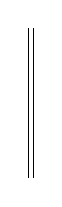
\begin{tikzpicture}
\draw (0,0)--(0,1.9); \draw (.07,0)--(.07,1.9);
\end{tikzpicture}}

\mspage{141}

\scanpage{143}
\mspage{480}

Dans l'optique de la réflexion de ces derniers jours, c'est ce moment de retrouvailles avec mon enfance, crue perdue et morte une longue vie durant, qui marque la fin de la ``deuxième période'' de mon itinéraire spirituel: celle de la prédominance, dans ma vie personnelle, des m é c a n i s m e s é g o t i - q u e s, à l'encontre des forces créatrices, des forces de connaissance et de renouvellement, qui avaient passé par une stagnation presque complète de quarante ans.C'est aussi l'époque de la prépondérance d'une ``certaine force'', d'une force à caractère presque exclusivement ``viril'', à l'image des valeurs en \unsure{honneu|honneur} dans le monde environnant, aux dépens des aspects et forces profondes ``féminins'' de mon être, ignorés et refoulés (avec un succés jamais complet, Dieu merci!).

La toute première intuition sur la nature destructrice de cette force-là, laquelle avait dominé ma vie comme celle de ma mère, et celle d'autres femmes aussi qui avaient été importantes dans ma vie - cette intuition fait une courte apparition en ces jours de maturation intense, à la faveur sûrement du \unsure{ressurgis|ressurgis-}\newline sement de l'énergie yin, ``féminine'', dans mon appréhension consciente des \unsure{choses|choses.} Contrairement à ce dont je croyais hâtivement me souvenir tantôt, cette apparition n'a pas lieu dans la méditation de la veille des retrouvailles, mais quelques heures après celles-ci, dans une courte méditation sur le sens de ce qui venait de se passer. L'intuition naît et prend forme tout à la.fin des quelques pages de notes de cette méditation. Je perçois la nature destructrice de \unsure{ce|cet-}\newline te ``force'' (qu'aujourd'hui j'appellerais ``force superyang'', c'est à dire à dominante yang excessive) chez ma mère d'abord, puis chez d'autres femmes, pour \unsure{en|en-}chaîner avec ces lignes finales:

\begin{quote}
`` Quant à la ``force'' en moi-même, c'est elle certes qui a fait de moi la cible et l'objet, attendus une jeune vie durant, de la haîne secrète et du ressentiment de M., puis de J., puis de S. - d'une haîne déposée en elles longtemps avant qu'elles ne connaissent mon existence, en les jours désemparés d'une enfance privée d'amour.''
\end{quote}

Le mot ``enfance'', dans la dernière ligne encore qui témoigne d'un jour important entre tous dans ma vie, y apparaît d'ailleurs pour la dernière fois \unsure{pou|pour} près de trois ans! Quant à l'intuition sur la nature de la force superyang en moi, comme provocatrice de réactions antagonistes, voire de haîne et de ressentiment, elle a eu tendance (il me semble) à sombrer un peu dans l'oubli jusqu'à ces tout derniers jours encore. Plus précisément, elle est restée présente seulement dans ma perception de certaines relations importantes dans ma vie (et \unsure{su|sur-}\newline tout, des relations avec des femmes que j'ai aimées). Par contre, elle n'a \unsure{guèr|guère}

\mspage{142}

\scanpage{144}
\[
 E_1\otimes E_2^{\deleted{\unsure{*}}}
\]
\figure{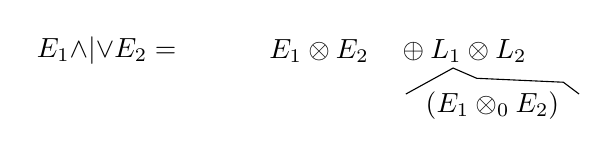
\begin{tikzpicture}
\node at (0,0) {$E_1\unsure{\wedge|\vee}E_2=$};
\node at (3.7,0) {$E_1\otimes E_2\quad\oplus L_1\otimes L_2$};
\node at (4.9,-.7) {$(E_1\otimes_0 E_2)$};
\draw (3.8,-.55)--(4.4,-.22)--(4.7,-.35)--(5.8,-.4)--(6,-.55);
\end{tikzpicture}}

$f_i$ endom de $E_i$ t.q. $\unsure{u_i|f_i}(L_i)\subset L_i$
\[
 \unsure{u_i|f_i}\big|_{L_i}=\unsure{u^!_i|f^!_i}:L_i\longrightarrow L_i
\]
\deleted{$u_2$ endom de $E_2$}
\[
 \begin{array}{lll}
 f_1\otimes f_2&\text{sur}&E_1\otimes E_2\\
 f^!_1\otimes f^!_2&\text{---}&L_1\otimes L_2
 \end{array}
\]
\[
 \deleted{u_1\otimes u_2}\qquad
 \begin{aligned}
 f(x_1*x_2)&=f_1(x_1)*f_2(x_2)\\
 f(u_1\otimes u_2)&=f^!_1(u_1)\otimes f^!_2(u_2)
 \end{aligned}
\]
\diagram{\begin{tikzcd}
 E_1\otimes L_2\arrow[dd]&\unsure{E_1\otimes E_2}&\\
 &x_1\otimes u_2\arrow[r,mapsto]&f_1(x_1)*f_2(u_2)\\
 x_1\otimes u_2\arrow[ur,mapsto]\arrow[dr,mapsto]&&\\
 &\pi_1(x_1)\otimes u_2\arrow[r,mapsto]&f^!_1(\pi_1(x_1))\otimes f^!_2(u_2)
\end{tikzcd}}
\[
 f_1(x_1)*v_2=f^!_1(\pi_1(x_1))\otimes v_2
\]
\[
 \deleted{\unsure{f(x_1}}\qquad\uline{\text{Ex}}\qquad f=
\]
\[
 f_1(x_1)=f_1(\pi\qquad \deleted{\unsure{f_2}}
\]
\diagram{\begin{tikzcd}
 E_1\otimes E_2\arrow[r]&\uline{\unsure{L_1|B_1}}\otimes L_2\\
 \alpha&\chi f_1\otimes f_2
\end{tikzcd}}
\[
 x_1-\pi_1(x_1)
\]
\diagram{\begin{tikzcd}
 E_1\arrow[d,"f_1"']&E_2\arrow[d,"f_2"]\\
 L_1&L_2\\
 \lambda_1&\lambda_2
\end{tikzcd}}
\figure{\begin{tikzpicture}\draw (0,0)--(0,2.5);\end{tikzpicture}}
\diagram{\begin{tikzcd}
 &E_1\otimes E_2\arrow[r]&L_1\otimes\unsure{L_2}\\
 E_1\otimes L_2\arrow[ur]\arrow[dr]& &\\
 &L_1\otimes L_2\arrow[uur,"{\deleted{\unsure{\chi f_1\otimes f_2}}\ \unsure{f^!_1f^!_2|f^!_1\otimes f^!_2}}"']&
\end{tikzcd}}
\[
 \begin{array}{cc}
 f_1&f_2\\[.5em]
 \lambda_1&\lambda_2
 \end{array}
\]
\[
 -\qquad \deleted{\unsure{f_1(}}\qquad x_1\otimes u_2\qquad
 \chi(\pi_1(x_1)\otimes u_2)
\]
\[
 \deleted{\lambda_1\lambda_2(\pi_1(x_1)\otimes u_2)}
\]
\[
 \deleted{f_1\otimes f_2}\qquad f_1(\pi_1(\unsure{x^!_1|x'_1}))\otimes f_2(u_2)
\]
\figure{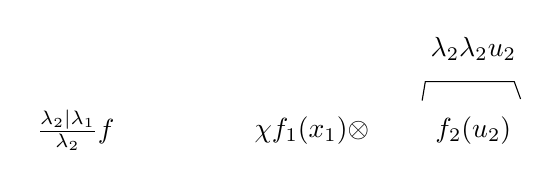
\begin{tikzpicture}
\node at (0,0) {$\frac{\unsure{\lambda_2|\lambda_1}}{\unsure{\lambda_2}}f$};
\node at (3,0) {$\chi f_1(x_1)\otimes$};
\node at (5.05,0) {$f_2(u_2)$};
\draw (4.4,.38)--(4.44,.62)--(5.57,.62)--(5.65,.40);
\node at (5.05,1.04) {$\deleted{\unsure{\lambda_2}}\lambda_2u_2$};
\end{tikzpicture}}
\[
 \deleted{\unsure{f_1(f^!_1(x_1)\otimes u_2}\ \unsure{\longrightarrow}}
\]
\[
 \lambda_1\deleted{\unsure{\lambda_2}}\pi_1(x_1)\otimes\unsure{\lambda_2u_2}
\]
\[
 \deleted{\lambda_2f_1(x_1)=\lambda}
\]
\[
 \lambda_1\pi_1(x_1)=f_1(x_1)\chi
\]
\mspage{143}

\scanpage{145}
\mspage{474}

pourtant plusieurs années, je crois, avant que je m'intériorise et ne reprenne \unsure{à} mon compte ces attitudes là, comme la honte de me montrer nu, allant de pair \unsure{ave|avec} une relation ambigüe avec mon corps. Cette honte,inculquée dès le jeune âge, est un des aspects d'une division profonde, où le corps est objet d'un tacite \unsure{mépris|mépris,} alors que les valeurs dites ``culturelles'' (confondues avec des capacité \unsure{intellec|intellec-}\newline tuelles de mémorisation et autres) sont montées en épingle. Cette division en mo\inserted{i} est restée ignorée jusqu'à ma quarante-huitième année, où elle a commencé à se \unsure{ré}\inserted{-}\newline soudre. C'est là le deuxième grand tournant de ma vie, qui marque l'avènement \unsure{de} la ``troisième période'' dans l'histoire de ma relation à moi-même, c'est-à-dire \unsure{a|aus-}\newline si celle de ma relation à mon corps, et à ``l'homme'' et à ``la femme'' en moi. \unsure{Mais} auparavant j'ai eu ample occasion de contribuer à transmettre cette\unsure{-| }division à mes enfants (*)\inserted{,} que j'ai pu voir la transmettre à leur tour...

J'ai fait allusion déjà hier (**) au ``basculement'' qui a fini par avoir lieu en moi. Avec un décalage de plus de deux ans après l'arrachement au milieu familial initial (ou pour mieux dire, après la d e s t r u c t i o n de ce milieu), ce basculement consacre la mise en place des mécanismes répressifs courants, dont mon enfance avait eu la rare chance d'être exempte jusque là. J'ai détecté jusqu'à présent deux grandes forces de nature répressive, qui ont dominé ma vie d'adulte et une grande partie de mon enfance $({}^{108}1)$. Je crois pouvoir \unsure{dire} que leur apparition ne s'est pas faite progressivement, mais que dans mon cas ce\inserted{s} mécanismes sont apparus plus ou moins du jour au lendemain et dans toute leur force, comme conséquence d'un c h o i x délibéré, au niveau inconscient. J'a\inserted{i} qualifié précédemment ce choix d'``abdication'', mais en même temps c'était aussi un puissant principe d'action: le ``je serai comme ``eux'''' (et pas ``comme moi'') signifiait aussi: je vais ``miser'' sur ``la tête'', pas plus mauvaise chez moi que chez quiconque après tout, et me battre et ``les'' battre avec leurs propres \unsure{armes|armes.}

L'un de ces mécanismes, et celui qui m'interesse surtout ici, est un des plus communs qui soit: c'est la r é p r e s s i o n d e m e s \unsure{t r a i t|t r a i t s} ``f é m i n i n s'' (ou ceux ressentis comme tels par les consensus courants), au profit de valeurs ``viriles''. L'endroit de la médaille était bien sûr l'\unsure{inverstis|inverstis-}\newline sement à fond sur mes traits et aptitudes ressentis comme ``virils'' et le dévelop\inserted{-}\newline pement à outrance de ceux-ci, qui ont pris une place démesurée.

\figure{\begin{tikzpicture}\draw (0,0)--(3,0);\end{tikzpicture}}

(*) Du moins, aux quatre parmi eux que j'ai contribué à élever. Le cinquième et dernier est élevé par sa mère, et jusqu'à présent il ne s'est pas présenté une occasion propice pour seulement faire connaissance, lui et moi.

(**) Voir les débuts de la note précédente ``Eclosion de la force - ou les épousailles'', note n° \unsure{107|109}.

\mspage{144}
